\section{Empirical Studies}
\label{sxn:empirical}

In this section, we present empirical results. 
Our goals are to justify key technical claims, including key assumptions underlying our \SETOL approach, and to illustrate the behavior of \SETOL with respect to various parameters and hyperparameters.
Importantly, it is \emph{not} our goal to demonstrate that layer PL exponent~\ALPHA~and~\ALPHAHAT~perform well for diagnostics and predicting model quality for SOTA NN models, as that has been demonstrated previously~\cite{MM20a_trends_NatComm,MM21a_simpsons_TR,YTHx22_TR}.
% (using just the \HTSR \Phenomenology).

Since the \SETOL theory presented in Section~\ref{sxn:matgen} is (effectively) a single layer theory,
in order to carefully test (as opposed to simply use) \SETOL, we need to limit the degree of inter-layer interactions present in the model.
%%(For example, in one series of experiments, described below, all layers in the model are trained; and we then compare and contrast this with the case where only one layer was trained, and all other layers remained frozen with their random initializations.) 
To do so, we consider a three-layer \MultiLayerPerceptron (MLP3), trained on MNIST~\cite{MNIST1998}. 
We refer to the hidden layers as ``FC1 and ``FC2. Their output sizes and parameter counts are shown in 
Table~\ref{tab:mlp3}.

\begin{table}[h]
\begin{center}
        \begin{tabular}{| c | c | c | c |}
                \hline
                Layer & Units & Weight Parameters           & $\%$ of total \\ \hline \hline
                FC1   &   300 & $768 \times 300 = 230,700$  & $88.2\%$      \\ \hline
                FC2   &   100 & $300 \times 100 = 30,000$   & $11.4\%$      \\ \hline
                out   &    10 &  $10 \times 100 = 1000$     & $0.38\%$      \\ \hline
        \end{tabular}
\end{center}
\caption{Dimensions of each FC layer in the MLP3 model, along with weight matrix parameter count and fraction of the 
total.}
\label{tab:mlp3}
\end{table}

The following are the main topics we consider.

\begin{enumerate}[label=6.\arabic*]
\item
\textbf{\ModelQuality: \HTSR \Phenomenology.}
The \HTSR \Phenomenology provides a metric of model quality in the form of the PL exponent $\alpha$.%
\footnote{Prior work has shown that the \ALPHAHAT metric $(\hat{\alpha})$ accurately describes variations in model 
quality as a function of architecture changes~\cite{MM21a_simpsons_TR}. Since we do not vary the depth of the model in 
our evaluations, the \ALPHA metric ($\alpha$) is of interest in this setting.} 
In particular, smaller values of $\alpha$ (e.g., 
%%provided $\alpha$ is not spuriously low, as discussed in Section~\ref{sxn:HT_ESDs}, then 
values of $\alpha$ closer to $2$ than $3$ or $4$) should correspond to better models, e.g., having smaller test errors; and
a minimal error should be obtained when $\alpha=2$.
See Section~\ref{sxn:empirical-test_acc}.
\item 
\textbf{\EffectiveCorrelationSpace.}
The \SETOL theory is based on the notion of an \EffectiveCorrelationSpace, in which the learning and generalization occurs. 
This is the low-rank subspace $\mathbf{W}^{\EFF}$ of each layer $\mathbf{W}$ that approximates the teacher $\mathbf{T}$.
In particular, 
our measure of model quality should be restricted to $\mathbf{W}^{\EFF}$.
The \EffectiveCorrelationSpace can be identified from the tail of the ESD, $\rho_{tail}(\lambda)$, and it can be chosen according to one of several related Model Selection Rules.
See Section~\ref{sxn:empirical-effective_corr_space}.
\item 
\textbf{Evaluating the \TRACELOG  Condition.}
In the \HTSR \Phenomenology, when a model is very well-trained, the layer PL exponent $\alpha\simeq 2$.
In the \SETOL theory, when a model is very well-trained, the eigenvalues in the tail will satisfy the Empirical \TRACELOG  Condition, given in \EQN~(\ref{eqn:detX}).
% because its easier to interpret numerically. I checked and this (was) the only place where this equation was 
% referenced, so I added another reference in the Section itself.}
In Section~\ref{sxn:empirical-trace_log}, we provide a detailed analysis of this effect.
\item
\textbf{Computational Model Qualities.}
In Section~\ref{sxn:empirical_comp_r_transforms}, we empirically compare the HTSR layer-quality exponent $\alpha$ against the computational \RTransform-derived metric $\QT$ on fully trained MLP3 models. We show that for the FC1 layer, $\QT$ closely tracks $\alpha$ with small error bars and the expected batch-size trend, whereas for FC2, $\QT$ exhibits much larger variability—demonstrating that $\alpha$ provides a more stable and robust measure of layer quality.  
\item
\textbf{\CorrelationTraps.}
Recall, from Section~\ref{sxn:Traps}, that if a layer weight matrix $\mathbf{W}$ has a \CorrelationTrap
(and, in particular, those arising from SGD training with very large learning rates)
then it is likely that the test (and train) accuracy will be degraded, and $\alpha$ will drop below its optimal value. 
See Section~\ref{sxn:empirical-correlation_trap} for an empirical demonstration of this.
\item 
\textbf{Overloading and Hysteresis Effects.}
The experiments described so far validate that \SETOL makes valid predictions in the $\alpha \gtrsim 2$ range.
Beyond that point, \SETOL only predicts ``atypicality, in the sense of spin glass theory~\cite{nishimori01}. 
See Section~\ref{sxn:hysteresis_effect} for an examination of how the MLP3 behaves when it is pushed further out of that range of validity, e.g., by training only one layer, while keeping the others frozen. In particular, we compare results when a single layer is either over- vs under-parameterized.
\end{enumerate}

\noindent
We trained the MLP3 model independently, using both the Tensorflow 2.0 framework (using the Keras api, and on Google Colab) and pytorch, with the goal of consistent, reproducible results.
Each setting of batch size, learning rate, and trainable layer was trained with $5$ separate starting random seeds, and error bars shown in plots below represent one standard deviation taken over these $5$ random seeds. 
Each training run used the same early stopping criteria on the train loss: training was halted when train loss did not decrease by more than $\Delta E_{train}=0.0001$, over a period of $3$ epochs. 
In doing so, each model was trained with a different number of epochs; and, at the end, the best weights were chosen for the model.
See Appendix~\ref{sxn:appendix_MLP3details} for more details on the MLP3 model and the training setup.
We provide a Google Colab notebook with the exact details, allowing the reader to reproduce the results as desired.

\michael{MM TO DO: make sure the following comment is mentioned earlier, not here.}
The dominant generalizing components of $\mathbf{W}$ reside in $\mathbf{W}^{\EFF}$ such that it captures the functional contribution of $\mathbf{W}$ to the NN; and thus
\charles{FINISH THOUGHTS HERE}



\subsection{\HTSR Phenomenology: Predicting Model Quality via the \ALPHA metric}
\label{sxn:empirical-test_acc}

\begin{figure}[t]
  \center
  \subfigure[Batch size experiment]{
    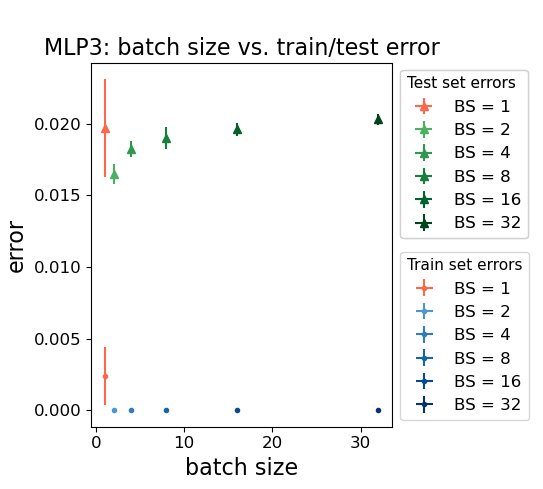
\includegraphics[width=6cm]{img/model_quality/mlp3_error_by_BS.png}
    \label{fig:mlp3-accuracies-bs}
  }
  \subfigure[Learning rate experiment]{
    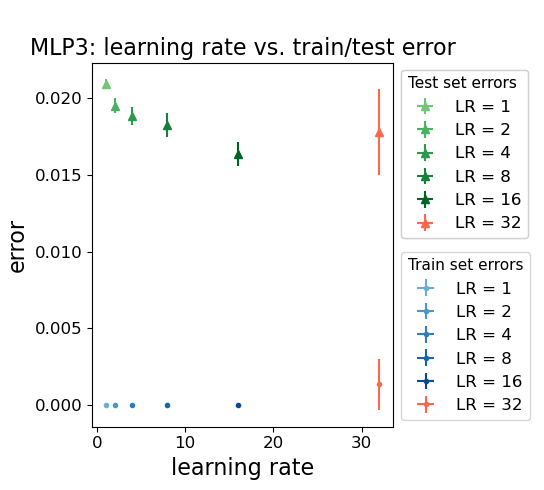
\includegraphics[width=6cm]{img/model_quality/mlp3_error_by_LR.png}
    \label{fig:mlp3-accuracies-lr}
  }
  \caption{Train / test errors in the MLP3 model as a function of batch size, and learning rate. Observe the inverse relationship between batch size (a) and learning rate (b). As batch size decreases, test error generally decreases, until batch size reached $bs=1$. Similarly, as learning rate increases, test error decreases until $lr=32\times$ the SGD default value of $0.01$.
  }
  \label{fig:mlp3-accuracies}
\end{figure}

Here, we want to determine how the quality of our MLP3 model varies with the \ALPHA metric. 
From previous work~\cite{MM20a_trends_NatComm,MM21a_simpsons_TR,YTHx22_TR}, we expect that \ALPHA metrics for the FC1 and FC2 layers should be well-correlated with the test accuracy, while varying some suitable training knob, such as learning rate or batch size, that can modulate the test accuracy.% 
\footnote{Since we do not change the depth of the model here, we expect the \ALPHA metric to follow the \ALPHAHAT metric, also predicting the test accuracies~\cite{MM21a_simpsons_TR}.}

In doing this, the goal is not to achieve \Thermodynamic equilibrium,
but, instead, by using a common stopping rule, to simulate 
in more realistic situations where models may not have fully converged.   This  allows us to test the theory outside of
its more limited apparent range of validity, 
thereby demonstrating the robustness of \SETOL.

We vary the batch size from small to large, i.e., $bs\in[1,2,4,8,16,32]$, following the setup of previous work on the \HTSR~\Phenomenology~\cite{MM18_TR_JMLRversion}. 
We expect similar effects by varying the learning rate, as it is known that small batch sizes correspond directly to large learning rates~\cite{SKYL17_TR,WT11}. 
Thus, we conducted a second set of experiments where the learning rate was varied by a factor of 
$[1\times,2\times,4\times,8\times,16\times,32\times]$, relative to the SGD default value of $0.01$. 
Adjusting the learning rate or batch size allows us to systematically vary the layer PL exponent $\alpha$ between roughly $2$ and $4$, i.e., within the range in which \SETOL should make the most reliable predictions. 
As an added benefit, it also allows us to use the very small batch size of $1$ to force the model into a state of over-regularization, which we also analyze below.


%%(In the HTSR \Phenomenology and the $5+1$ Phases-of-Training, and with how \WW~currently fits the ESDs, and barring additional spurious effects, this over-fitting regime corresponds to \VeryHeavyTailed (VHT) ESDs, with $\alpha<2$, which corresponds to a different HT \Universality class than $\alpha \in [2,4]$~\cite{MM18_TR_JMLRversion}.)

Consider Figure~\ref{fig:mlp3-accuracies}, which plots the final train and test accuracies as a function of the hyperparameter (batch size or learning rate) used during training for the MLP3 model.
Figure~\ref{fig:mlp3-accuracies-bs} varies batch size, and Figure~\ref{fig:mlp3-accuracies-lr} varies learning rate.
Recall that error bars represent one standard deviation taken over $5$ independent starting random seeds. 
In Figure~\ref{fig:mlp3-accuracies-bs}, we see that by decreasing the batch size ($bs$), and holding other knobs constant, we can systematically improve the train and test accuracy, up to a point. 
In particular, for $bs \ge 2$, both the test and train accuracies increase with decreasing batch size, consistent with previous work~\cite{MM18_TR_JMLRversion}.
Further decrease beyond $bs=2$ leads to \emph{lower} model quality, i.e., larger error and larger error variability.
In Figure~\ref{fig:mlp3-accuracies}, we see that increasing the learning rate ($lr$) by a factor $x$ has an exactly analogous effect as decreasing the batch size by $1/x$.% 
\footnote{One could, of course, mitigate this by fiddling with other knobs of the training process, but that is not our goal.  Our goal here is not to use a toy model to demonstrate the properties and predictions of \SETOL.}

\begin{figure}[t]
    \centering
    \subfigure[$\alpha_{FC1}$]{
        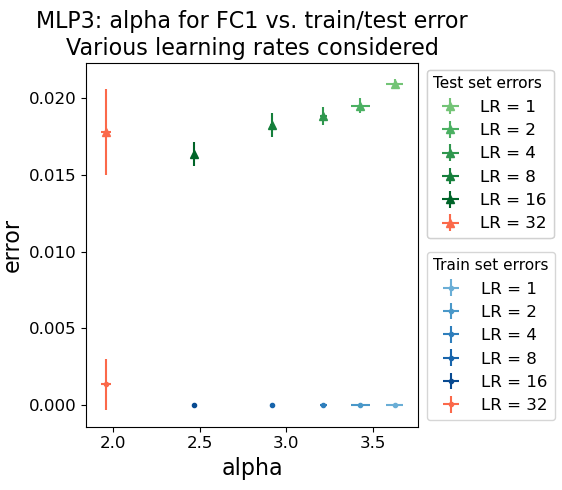
\includegraphics[width=6cm]{img/model_quality/mlp3_alpha_FC1_by_LR.png}
        \label{fig:mlp3-alpha-fc1-by-lr}
    } 
%    \subfigure[$\Delta \lambda_{min}$ FC1]{
%        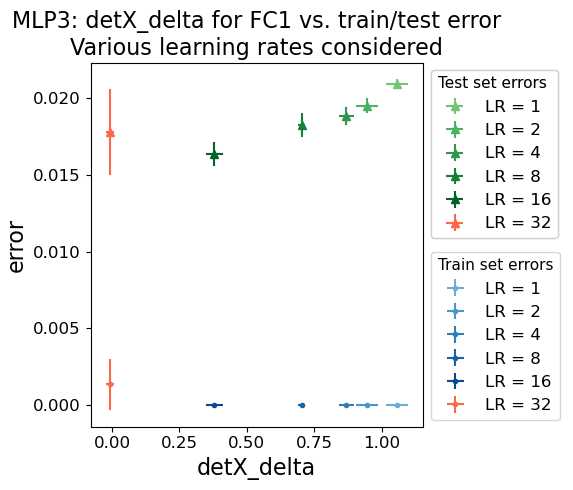
\includegraphics[width=6cm]{img/model_quality/mlp3_detX_Delta_FC1_by_LR.png}
%        \label{fig:mlp3-detx-delta-fc1-by-lr}
%    } \\
    \subfigure[$\alpha_{FC2}$]{
        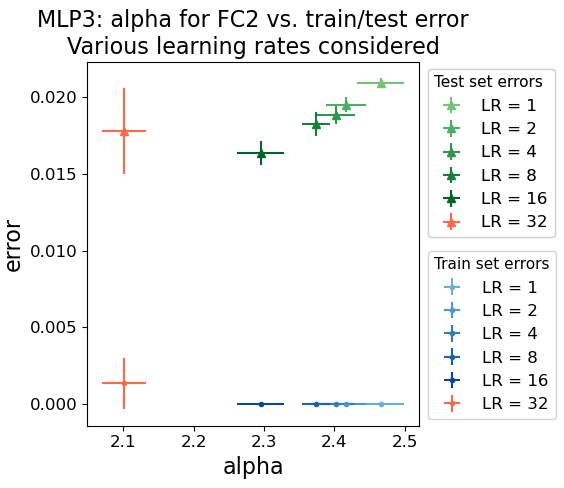
\includegraphics[width=6cm]{img/model_quality/mlp3_alpha_FC2_by_LR.png}
        \label{fig:mlp3-alpha-fc2-by-lr}
    } 
%    \subfigure[$\Delta \lambda_{min}$ FC1]{
%        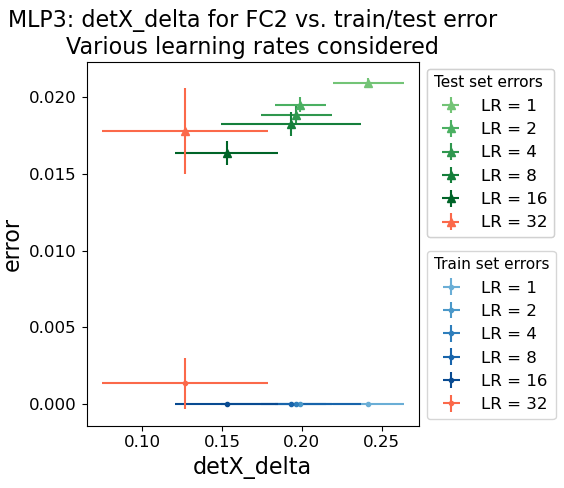
\includegraphics[width=6cm]{img/model_quality/mlp3_detX_Delta_FC2_by_LR.png}
%        \label{fig:mlp3-detx-delta-fc2-by-lr}
%    }  

    \caption{
            Train / test errors in the MLP3 model in the {\bf \emph{\LearningRate}} experiment as a function of $\alpha_{FC1}$ (a) and $\alpha_{FC2}$ (b). 
            Observe the regular downward progression of $\alpha$ and error as the learning 
            rate increased in both (a) and (b). When learning rate was $32\times$, (shown in red), $\alpha_{FC1}$ fell 
            below $2$, coinciding with a drastic increase in both train and test error. The results here almost 
            perfectly replicate those of the Batch Size experiment, shown in Figure~\ref{fig:mlp3-alphas-bs}.
              for Figure~\ref{fig:mlp3-alphas-bs}.}
 \label{fig:mlp3-alphas-lr}
\end{figure}

The transition between $lr=16\times$ (or $bs=2$), which is locally optimal for the setting of other hyperparameters, and $lr=32\times$ normal (or $bs=1$), which is not, provides a demonstration of a distinct change in the behavior of \ALPHA, concordant with the sudden increase in the error and error variability. 
To explore this in the context of \SETOL, consider Figure~\ref{fig:mlp3-alphas-lr} and Figure~\ref{fig:mlp3-alphas-bs}, which plot error as a function of \ALPHA, for different learning rates and batch sizes, respectively.

Figure~\ref{fig:mlp3-alphas-lr} plots the \ALPHA metrics $\alpha_{FC1}$ and $\alpha_{FC2}$, as learning rate is varied, demonstrating that both metrics are well-correlated with the test accuracies, for all learning rates less than $16\times$ normal. 
In particular, as we drive \ALPHA in FC1 down to an \Ideal value of $\alpha\simeq 2$, the test error decreases monotonically (Figure~\ref{fig:mlp3-alpha-fc1-by-lr}).
Beyond that point, further decrease of the batch size sees \ALPHA decrease below its \Ideal value of $2$ in the FC1 layer.
This corresponds not only with \emph{higher errors}, but also with \emph{larger error bars}, on both train and test error. 
The dramatic increase in train error and train error variability is particularly telling, because it suggests that when 
$\alpha_{FC1}$ passes below $2$, the model enters into a ``glassy state, and is unable to relax down to $0$ train error.

In Figure~\ref{fig:mlp3-alpha-fc2-by-lr}, we consider \ALPHA for FC2, and we see that $\alpha_{FC2}$ approaches $2$, but 
does not reach it, even for $lr=32\times$. This failure to achieve $\alpha_{FC2} \approx 2$, along with the much greater size 
of FC1, (See Table~\ref{tab:mlp3},) suggests that FC1 is the critical layer for the models performance. 
This also highlights some of the interplay between the layers, (which is not captured by a single layer theory) -- as $\alpha_{FC1}$ has narrow error bars throughout, $\alpha_{FC2}$ shows much more variation by way of its wider error bars. 
Thus, while model accuracy kept improving as learning rate increased up to $16\times$, this was likely driven by a better $\alpha_{FC1}$, more than by $\alpha_{FC2}$. 

In Figure~\ref{fig:mlp3-alphas-bs}, we consider batch size, and we see a near identical replication of these results, in terms of the relation of train error, test error and \ALPHA in the two layers. 
Consequently, the remainder of the experiments will focus on the learning rate experiment, as both produced substantially the same results.

\begin{figure}[t] %[h]
    \centering
    \subfigure[$\alpha_{FC1}$]{
        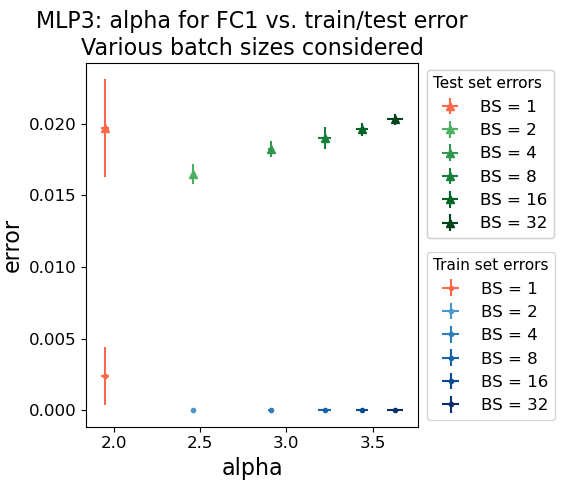
\includegraphics[width=6cm]{img/model_quality/mlp3_alpha_FC1_by_BS.png}
        \label{fig:mlp3-alpha-fc1-by-bs}
    } 
%    \subfigure[$\Delta \lambda_{min}$ FC1]{
%        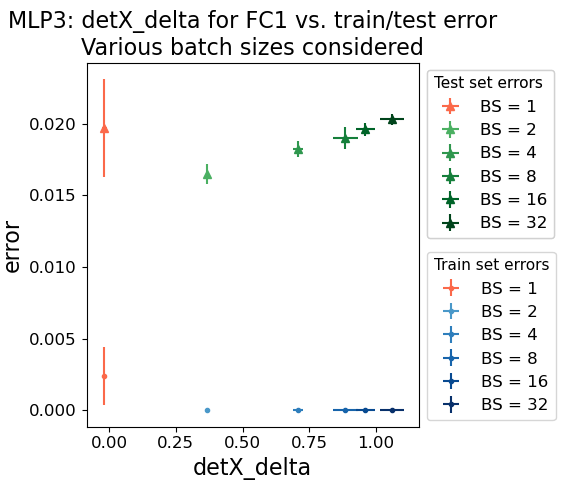
\includegraphics[width=6cm]{img/model_quality/mlp3_detX_Delta_FC1_by_BS.png}
%        \label{fig:mlp3-detx-delta-fc1-by-bs}
%    } \\
    \subfigure[$\alpha_{FC2}$]{
        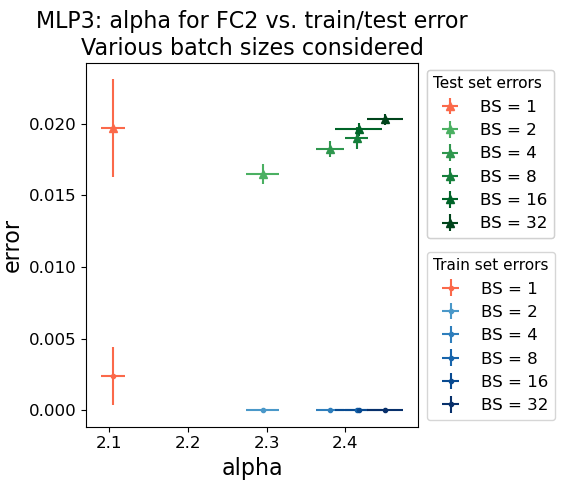
\includegraphics[width=6cm]{img/model_quality/mlp3_alpha_FC2_by_BS.png}
        \label{fig:mlp3-alpha-fc2-by-bs}
    } 
%    \subfigure[$\Delta \lambda_{min}$ FC1]{
%        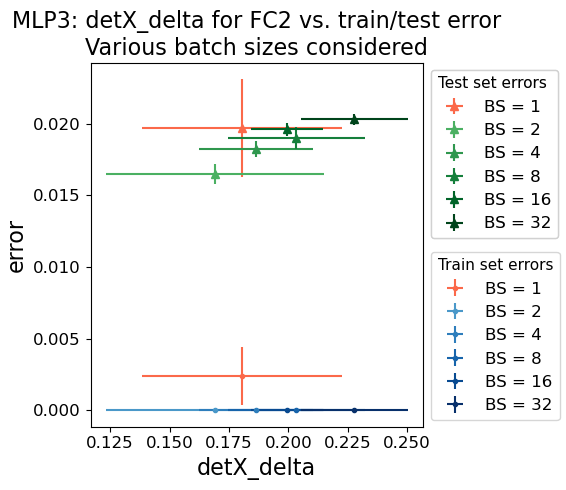
\includegraphics[width=6cm]{img/model_quality/mlp3_detX_Delta_FC2_by_BS.png}
%        \label{fig:mlp3-detx-delta-fc2-by-bs}
%    }  

    \caption{
            Train / test errors in the MLP3 model in the {\bf Batch Size} experiment as a function of $\alpha_{FC1}$ 
            (a) and $\alpha_{FC2}$ (b). Observe the regular downward progression of $\alpha$ and error as the batch size
            decreased in both (a) and (b). When batch size was $1$, (shown in red), $\alpha_{FC1}$ fell below $2$, 
            coinciding with a drastic increase in both train and test error. The results here almost perfectly 
            replicate those of the \LearningRate experiment, shown in Figure~\ref{fig:mlp3-alphas-lr}.
    }
 \label{fig:mlp3-alphas-bs}
\end{figure}





\subsection{Testing the Effective Correlation Space}
\label{sxn:empirical-effective_corr_space}

Here, we will address the question: 
\begin{quote}
How shall we \emph{test the assumption} of the \EffectiveCorrelationSpace?
\end{quote}
Recall that the \SETOL theory estimates model quality by evaluating the ST \GeneralizationError as an integral over the theoretical training data $\boldsymbol{\xi}$.
This integral assumes each layer weight matrix can be replaced with an effectively lower rank form, i.e., $\mathbf{W}\rightarrow\mathbf{W}^{\EFF}$, corresponding to the span of the eigencomponents defined by the tail of the ESD, $\rho_{tail}(\lambda)$. 
In the \HTSR \Phenomenology, the tail is defined by the fact that $\rho_{tail}(\lambda)$ follows a PL distribution, above some minimal value $\lambda_{min}$.
In our \SETOL theory, the tail is defined by choosing the minimal value $\lambda_{min}$ to satisfy the Empirical \TRACELOG  condition.
%
These methods of realizing $\mathbf{W}^{\EFF}$ are essentially \emph{Model Selection Rules} (MSRs) for the \EffectiveCorrelationSpace. 
%By ``\ModelSelectionRule, we refer to a procedure to choose a $\lambda_{min}$ such that all eigenvalues above $\lambda_{min}$ are included in the tail. 
%
Importantly, in neither approach is $\lambda_{min}$ just some ``rank parameter to be chosen by yet some other MSR on 
the basis of rank, or magnitude alone, (that, in particular, does not know about \HTSR or \SETOL, which consider the 
\emph{shape} of the ESD).

Thus, to test the assumption of the \EffectiveCorrelationSpace, we want to show that the models predictions are in fact controlled predominantly by the tail, where the specific choice of the rank parameter depends on \HTSR or \SETOL as we expect.
We can emulate this theoretical construct and estimate (trends in the) test accuracies by evaluating the train and/or 
test accuracies of the trained MLP3 model -- after replacing the MLP3 layer weight matrices $\mathbf{W}_{FC1}$ and $\mathbf{W}_{FC2}$ with a low-rank approximation consisting of \emph{only} the tail:
% using a TruncatedSVD method:
\begin{align*}
 \mathbf{W}^{\EFF}_{FC1}:= P_{tail}\mathbf{W}_{FC1} \\
 \mathbf{W}^{\EFF}_{FC2}:= P_{tail}\mathbf{W}_{FC2}  ,
\end{align*}
where $P_{tail}$ is a projection operator selecting only the tail of the ESD with TrucnatedSVD.
(That is, we will use the  low-rank TruncatedSVD approximation at the inference step, not at the training step, as is more common.)
A Truncated model is one whose weight matrices $\mathbf{W}_*$ have been replaced by truncated matrices $\mathbf{W}^{\EFF}_*$. 
We denote the difference between the original models accuracy and the Truncated models train and test accuracy as $\Delta E_{train}$ and $\Delta E_{test}$, respectively:
\begin{align*}
  \Delta E_{train}:=  E_{train}(\mathcal{D}) - E^{\EFF}_{train}(\mathcal{D}) \\
  \Delta E_{test}:=  E_{test}(\mathcal{D}) - E^{\EFF}_{test}(\mathcal{D})  ,
\end{align*}
where $E^{\EFF}_{train}$ denotes the error of the TruncatedSVD model on the training portion of the dataset $\mathcal{D}$,a
and  $E^{\EFF}_{test}$ denotes corresponding test error for the TruncatedSVD model.
%$\Delta E$ denotes the difference between test and/or training accuracies (for difference batch sizes $bs$).

\paragraph{The \POWERLAW~and \TRACELOG~Model Selection Rules}
\charles{is MSR still a good theme here?  In the orginal paper we discussed the MSR up front. Now
  we seem to just casually mention it here.}
If we use good MSRs, then we expect that $\Delta E_{train}\to 0$ and $\Delta E_{test}\to 0$ as the models approach \IdealLearning. 
%
We consider the following MSRs,%
\footnote{We considered other MSRs that do not ``know about \HTSR or \SETOL, but they (expectedly) perform in trivial or uninteresting ways for testing the assumption of the \EffectiveCorrelationSpace.  Thus, we are not introducing just some arbitrary low-rank approximation, as is common, but instead that the specific \SETOL-based MSR matters.} 
which are associated with the \HTSR and \SETOL approaches.
\begin{itemize}
\item 
The \POWERLAW~MSR: 
All eigenvalues lying in the tail of the ESD, 
$\lambda_i \ge \LAMBDAPL$, where $\LAMBDAPL$ is the start of the PL tail, as determined by the \WW~PL fit, which is based on \cite{CSN09_powerlaw}.
\item 
The \TRACELOG~MSR: 
All eigenvalues lying in the tail of the ESD, 
such that they satisfy the \TRACELOG  Condition, i.e., $\lambda_{i}\ge \LAMBDADETX$, where $\prod\lambda_{i:\lambda_i \ge \LAMBDADETX}\simeq 1$.
\end{itemize}
\chris{CH TODO: Find a place to call out the need for Normalizing $W$ to Frobenius norm = $M$.}


%\chris{I commented out the part about Kendals tau rank statistics. Lets discuss if we would like to add it back in}
%The MSRs lead directly to data-dependent quality metrics. By this, 
%we mean metrics that directly evaluate the train error of the model,
%using the actual training data $\mathcal{D}$, and with either the unmodified (i.e. bare)
%or some modified (i.e effective, smoothed)  model.  
%
%Then, we can compare and contrast the different MSRs in order to
%see how well they can predict the trends in the test accuracies
%for the different batch sizes.
%We do this visually and by computing the rank correlation 
%between the actual $E_{test}$ and predicted $E^{\EFF}_{train}(\mathcal{D})$
%(i.e. with the Kendall-tau rank correlation metric).

%\item The \SVDA~and \SVDB MSRs:  The \SVDA retains the top $20\%$ of the eigenvalues of the tail of the ESD, and the \SVDB~MSR retains the  top $40\%$.
%For all MSRs, we apply the TruncatedSVD approximation to $\mathbf{W}$, keeping only those
%eigencomponenents associated with the eigenvalues in the tail. 


%\chris{There are 6 plots for each MSR, but I think showing 3 gets the point across. Just remove comments below to add 
%them back in.}


\subsubsection{Train and test errors by epochs}
\label{sxn:trunc_err_epochs}
\begin{figure}[t]
    \centering
    \subfigure[$lr=1\times$]{
        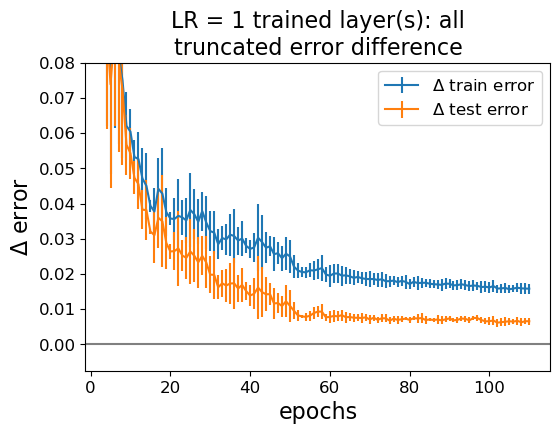
\includegraphics[width=5cm]{img/truncated_error/mlp3_trunc_error_by_epochs_LR_0_all_xmin.png}
        \label{fig:mlp3-trunc_err_epochs_xmin_1}
    }
    \subfigure[$lr=2\times$]{
        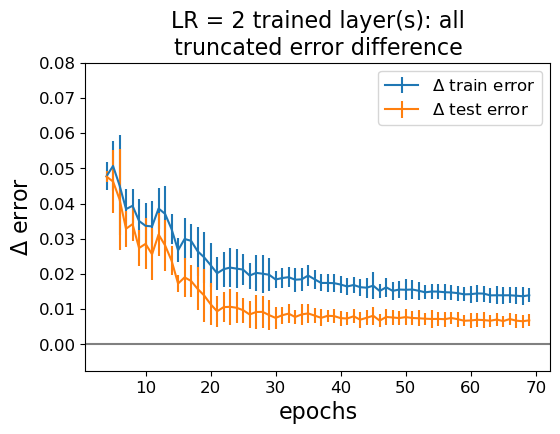
\includegraphics[width=5cm]{img/truncated_error/mlp3_trunc_error_by_epochs_LR_1_all_xmin.png}
        \label{fig:mlp3-trunc_err_epochs_xmin_2}
    }
    \subfigure[$lr=4\times$]{
        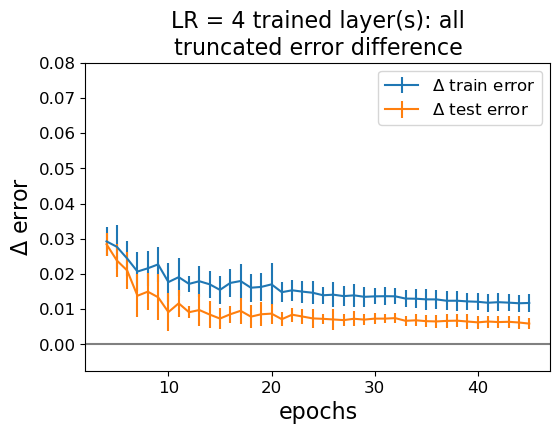
\includegraphics[width=5cm]{img/truncated_error/mlp3_trunc_error_by_epochs_LR_2_all_xmin.png}
        \label{fig:mlp3-trunc_err_epochs_xmin_4}
    }\\
    \subfigure[$lr=8\times$]{
        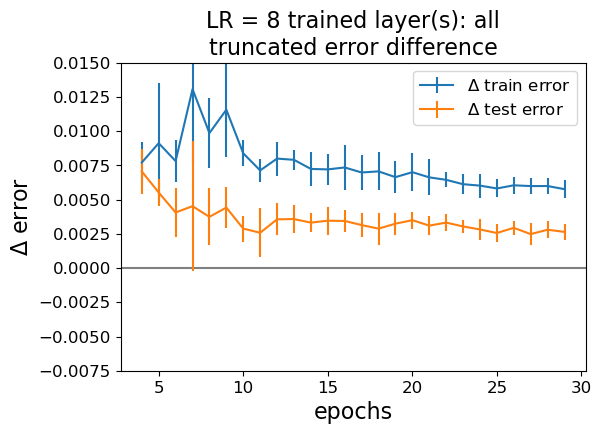
\includegraphics[width=5cm]{img/truncated_error/mlp3_trunc_error_by_epochs_LR_3_all_xmin.png}
        \label{fig:mlp3-trunc_err_epochs_xmin_8}
    }
    \subfigure[$lr=16\times$]{
        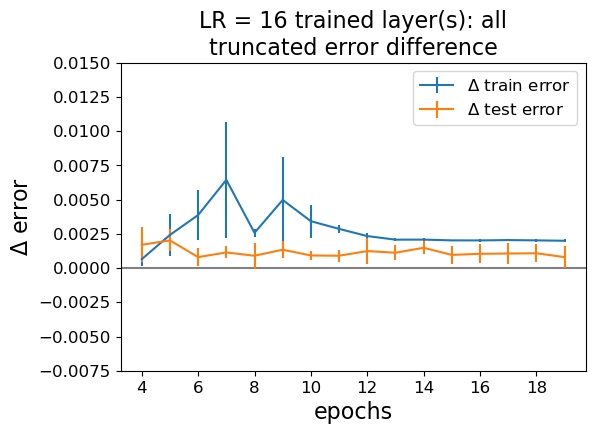
\includegraphics[width=5cm]{img/truncated_error/mlp3_trunc_error_by_epochs_LR_4_all_xmin.png}
        \label{fig:mlp3-trunc_err_epochs_xmin_16}
    }
    \subfigure[$lr=32\times$]{
        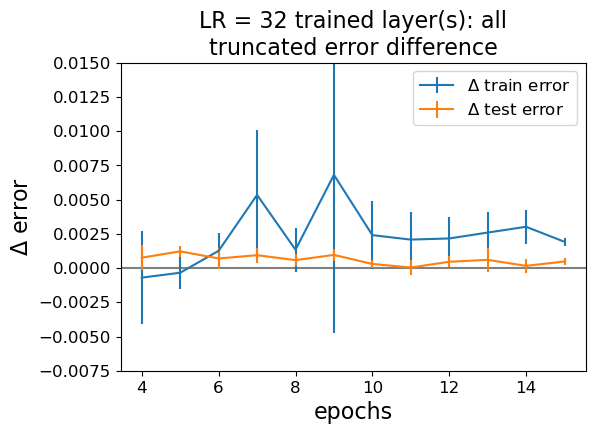
\includegraphics[width=5cm]{img/truncated_error/mlp3_trunc_error_by_epochs_LR_5_all_xmin.png}
        \label{fig:mlp3-trunc_err_epochs_xmin_32}
    }
    \caption{
            $\Delta E_{train}$ (blue) and $\Delta E_{test}$ (orange) for various learning rates, using the 
            \POWERLAW~MSR. As learning rate increases we can see that $\Delta E_{train}$ and $\Delta E_{test}$ both tend 
            towards lower asymptotic minima, which they reach after fewer epochs of training. We can also see that 
            (after the first few epochs,) $\Delta E_{train}$ (blue) is always higher than $\Delta E_{test}$ (orange). 
            Observe that in the bottom row (d--f) the yaxis is contracted to make the variation more visible. In (f) we can see 
            that as learning rate surpasses its optimal setting, the gap between $\Delta E_{train}$ and $\Delta 
            E_{test}$ begins to increase again, and has wider error bars, suggesting that the excessively large learning 
            rate is disrupting the MLP3s ability to lear the \EffectiveCorrelationSpace.
    }
    \label{fig:mlp3-msr-results-xmin}
    %Comparison of \POWERLAW~and \TRACELOG~ Model Selection Rules for testing the \EffectiveCorrelationSpace}
\end{figure}



To see how the \EffectiveCorrelationSpace forms, we plot how $\Delta E_{train}$ and $\Delta E_{test}$ evolve over training, for each of the various learning rates considered.%
\footnote{When batch size was varied, results did not significantly differ, and so they are omitted. 
%% CONFIRM WE HAVE SAID THIS ELSEWHERE %% See the experimental Colab notebooks for the full set of experiments.
} 

We start with the effect of the \POWERLAW~MSR.
See Figure~\ref{fig:mlp3-msr-results-xmin}, where we see that $\Delta E_{train}$ and $\Delta E_{test}$ generally trend 
downwards as they approach minimum train error. 
When the learning rate is larger, the models converge more quickly, and $\Delta E_{train}$ and $\Delta E_{test}$ also converge to lower values. 
Recall from Figure~\ref{fig:mlp3-accuracies-lr} that $lr=16\times$ had the lowest test error. In 
Figure~\ref{fig:mlp3-trunc_err_epochs_xmin_16}, we see that it also has the lowest $\Delta E_{train}$ and $\Delta 
E_{test}$. A lower $\Delta E_{train}$ or $\Delta E_{test}$ means that more of the models correct predictions are due to 
the low rank tail, meaning that the tail generalizes better, and we see here that when the tail generalizes best, the 
model was the most accurate. 

In each plot, we also see that the error bars are wide early on, before suddenly becoming much narrower. This transition 
is more visible in the larger learning rates shown in~\ref{fig:mlp3-trunc_err_epochs_xmin_8}--\ref{fig:mlp3-trunc_err_epochs_xmin_32},
but can also be seen in \ref{fig:mlp3-trunc_err_epochs_xmin_1}--\ref{fig:mlp3-trunc_err_epochs_xmin_4}, albeit less 
clearly. Most interestingly of all, this transition is preceded by a brief period, sometimes a single epoch, in which the 
error bars are drastically wider, in a way that is reminiscent of a first-order phase transition. Again, this 
phenomenon can be seen most clearly in ~\ref{fig:mlp3-trunc_err_epochs_xmin_8}--\ref{fig:mlp3-trunc_err_epochs_xmin_32}.


We next consider the effect of the \TRACELOG~MSR.
See Figure~\ref{fig:mlp3-msr-results-detX}, which also shows the development of $\Delta E_{train}$ and $\Delta E_{test}$ 
over epochs, where we see a very different pattern in the train error and test error. 
The difference in the train error is because, as the model is untrained in the early epochs, the \TRACELOG~MSR 
\emph{over}-estimates the tail by choosing a $\lambda_{min}$ that is too small. 
Thus, $\Delta E_{train}$ actually increases to its asymptotic value at the final epoch. 
In the earliest epochs, the truncated train error is even \emph{less} than the full MLP3 models error, suggesting that 
signal is forming in the large eigenvalues in these early epochs, but is swamped by the randomness of the early initial 
weights, some of which is then removed by truncation. As epochs progress, this effect disappears.
%
Here again we can see the ``phase-transition-like behavior of the train error, as the error bars are wide early on, up to a transition having an abnormally large error bar, after which they stabilize.

Perhaps most interestingly of all, we see that under the \TRACELOG Model Selection Rule (MSR), $\Delta E_{test}$ is flat \emph{throughout 
training}, and for all learning rates. This implies that there is \emph{no} point in training where the 
\TRACELOG tail generalizes badly. In other words, almost none of the out-of-sample variance falls outside of the \EffectiveCorrelationSpace, as the \TRACELOG~MSR over-estimates the \EffectiveCorrelationSpace. It also bears noticing that under the 
\POWERLAW~MSR, (Figure~\ref{fig:mlp3-msr-results-xmin},) this is decidedly not the case, because the \POWERLAW~MSR \emph{under}-estimates the \EffectiveCorrelationSpace. As we will see in \ref{sxn:empirical-trace_log}, as \ALPHA approaches $2$, the gap between the two MSRs goes to $0$.
%This means that a small, but 
%significant amount of generalization comes from the gap between these tails, but none at all %comes from the bulk.
%\nred{confusing}


\begin{figure}[t]
    \centering
    \subfigure[$lr=1\times$]{
        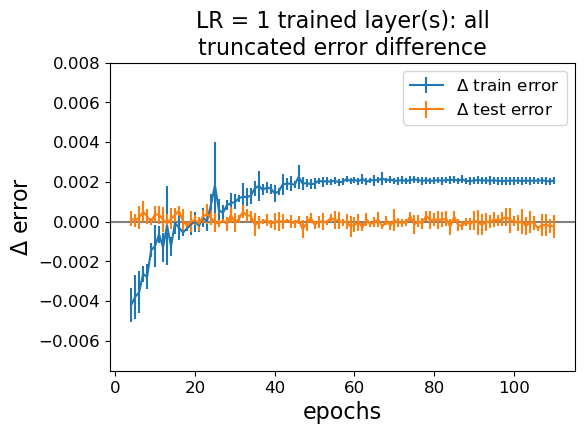
\includegraphics[width=5cm]{img/truncated_error/mlp3_trunc_error_by_epochs_LR_0_all_detX.png}
        \label{fig:mlp3-trunc_err_epochs_detX_1}
    }
    \subfigure[$lr=2\times$]{
        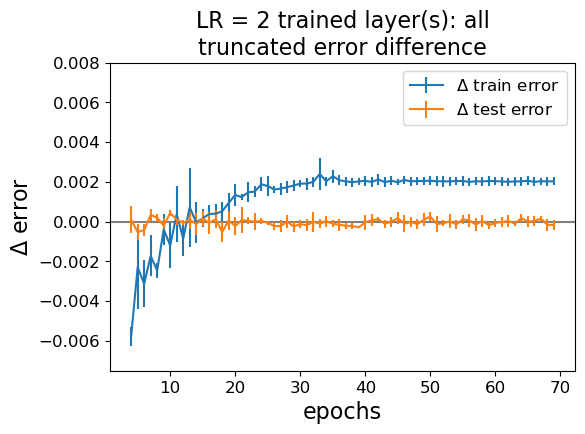
\includegraphics[width=5cm]{img/truncated_error/mlp3_trunc_error_by_epochs_LR_1_all_detX.png}
        \label{fig:mlp3-trunc_err_epochs_detX_2}
    }
    \subfigure[$lr=4\times$]{
        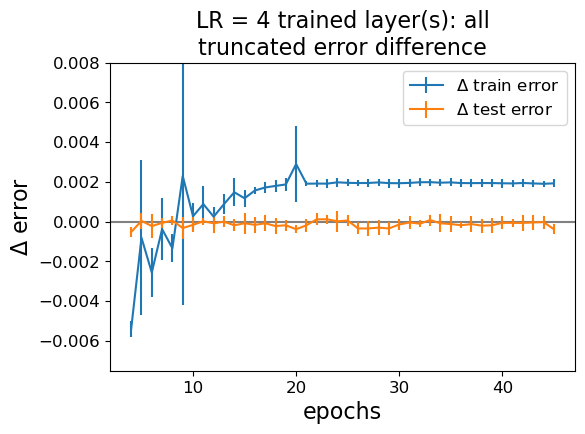
\includegraphics[width=5cm]{img/truncated_error/mlp3_trunc_error_by_epochs_LR_2_all_detX.png}
        \label{fig:mlp3-trunc_err_epochs_detX_4}
    }\\
    \subfigure[$lr=8\times$]{
        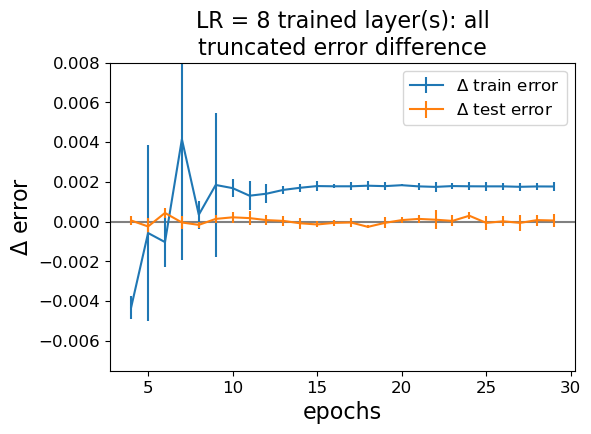
\includegraphics[width=5cm]{img/truncated_error/mlp3_trunc_error_by_epochs_LR_3_all_detX.png}
        \label{fig:mlp3-trunc_err_epochs_detX_8}
    }
    \subfigure[$lr=16\times$]{
        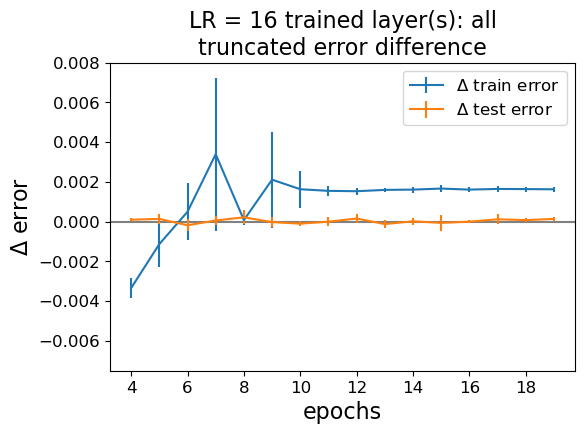
\includegraphics[width=5cm]{img/truncated_error/mlp3_trunc_error_by_epochs_LR_4_all_detX.png}
        \label{fig:mlp3-trunc_err_epochs_detX_16}
    }
    \subfigure[$lr=32\times$]{
        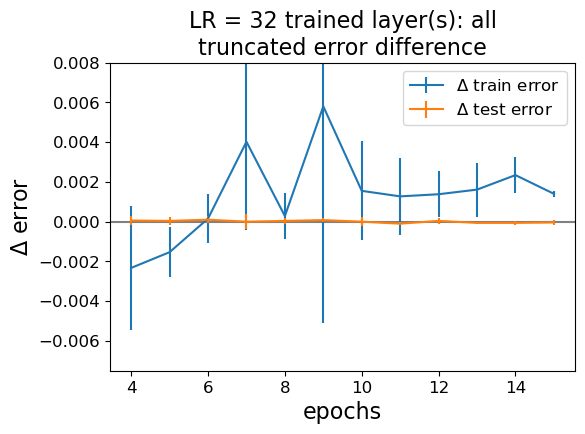
\includegraphics[width=5cm]{img/truncated_error/mlp3_trunc_error_by_epochs_LR_5_all_detX.png}
        \label{fig:mlp3-trunc_err_epochs_detX_32}
    }
    \caption{
        $\Delta E_{train}$ (blue) and $\Delta E_{test}$ (orange) for selected learning rates, using the \TRACELOG~MSR. 
        For all learning rates, $\Delta E_{test}$ is centered on $0$, meaning that the \TRACELOG~Effective Correlation 
        Space explains almost all variation in out-of-sample predictions, but it does \emph{not} explain all of the 
        training set predictions (blue). NOTE: The y axis is the same in all plots, and is much narrower than in 
        Figure~\ref{fig:mlp3-msr-results-xmin}. In (a--e) we can see that $\Delta E_{train}$ converges to approximately 
        $0.002$. Compare with Figure~\ref{fig:mlp3-trunc_err_epochs_xmin_16}, which reaches a minimum of approximately 
        $0.0025$. As in Figure~\ref{fig:mlp3-trunc_err_epochs_xmin_32}, the learning rate of $32\times$ normal disrputs the 
        MLP3s ability to discover the \TRACELOG \EffectiveCorrelationSpace.
    }
    \label{fig:mlp3-msr-results-detX}
    %Comparison of \POWERLAW~and \TRACELOG~ Model Selection Rules for testing the \EffectiveCorrelationSpace}
\end{figure}


There are two final points of comparison between Figures~\ref{fig:mlp3-msr-results-xmin} and~\ref{fig:mlp3-msr-results-detX}.
%
First, 
although it appears in Figure~\ref{fig:mlp3-msr-results-detX} that $\Delta E_{train}$ converges to a larger value than in Figure~\ref{fig:mlp3-msr-results-xmin}, this is because the scale of the y-axis is $10\times$ smaller. 
That is, the \POWERLAW~MSR is biased towards over-estimating $\lambda_{min}$, which means it over-truncates, producing a 
larger $\Delta E_{train}$ or $\Delta E_{test}$ 
than the \TRACELOG~MSR, which is biased towards under-estimating $\lambda_{min}$. 
%
Second,
in both Figure~\ref{fig:mlp3-msr-results-xmin} and~\ref{fig:mlp3-msr-results-detX}, we can see that $\Delta E_{test}$ is consistently lower than $\Delta E_{train}$. 
Clearly, truncating has a larger effect on train predictions, meaning that no matter how long the model is trained, some 
of the train predictions are still derived from the bulk. The fact that they remain is evidence that the gradient does not degrade them, meaning that they were most likely contributing spuriously correct answers. Yet, the test predictions are far less affected, meaning that only the \EffectiveCorrelationSpace contributes to the models ability to generalize.

\subsubsection{Truncation and Generalization}

%We can also estimate the test accuracies of the \emph{Truncated} models by evaluating the train accuracy of 
%\emph{Truncated} models
%\begin{align}
%  E_{test}\approx E^{\EFF}_{train}(\mathcal{D}) 
%\end{align}
%Generally speaking, this may not be as good of an approximation as above, but we
%can use this to study trends in the test accuracies for the \ALPHA and \ALPHAHAT metrics
%to see how \ALPHAHAT can correct for anamolously small alphas due to \CorrelationTraps.
Given that $\Delta E_{test}$ is always lower than $\Delta E_{train}$ for the \POWERLAW~MSR, and similarly for \TRACELOG~after a certain point in training, it is clear that the \EffectiveCorrelationSpace has something to do with generalization.
However, this leaves open the question of what role precisely \ALPHA plays. 
In Figure~\ref{fig:mlp3-alpha-generalization-gap}, we plot $\Delta E_{train}$ and $\Delta E_{test}$ with the \POWERLAW~MSR as a function of \ALPHA (rather than epochs) for layers FC1 and FC2, as well as the \GeneralizationGap -- that is, $E_{test} - E_{train}$. 
(Recall \EQN~\ref{eqn:gen_gap}.) 
Learning rate is not explicitly shown, but its effect can be seen in the clusters of points that each learning rate generates.

\begin{figure}[t]
  \centering
  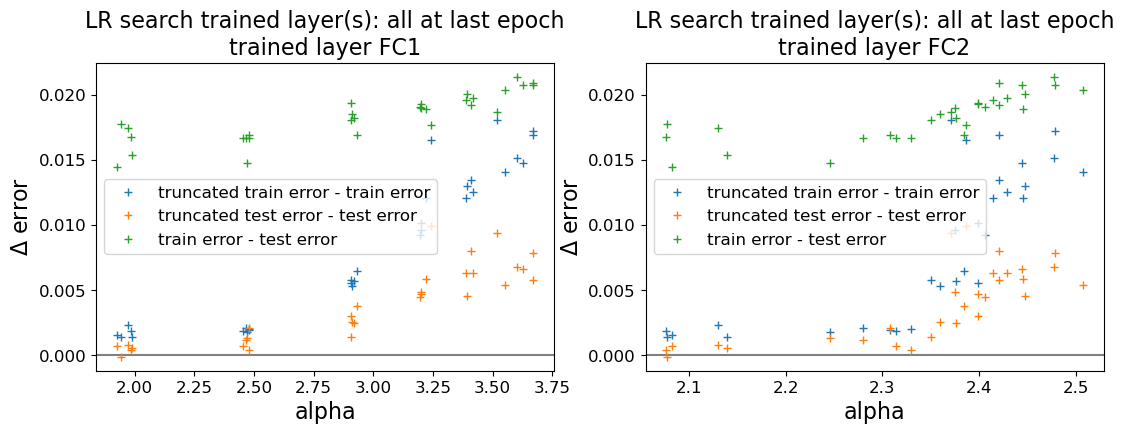
\includegraphics[width=15cm]{img/truncated_error/mlp3_trunc_error_by_LR_alpha_all_xmin.png}
  \caption{
        Train and test error gaps using the \POWERLAW~MSR, as a function of alpha in the FC1 and FC2 layers of MLP3 
        models, at the \emph{final epoch} of training. We can see that as alpha decreases towards $2$, (right to left), 
        $\Delta E_{train}$ and $\Delta E_{test}$ generally decrease as well, meaning that the closer $\ALPHA$ is to $2$, 
        the more the Effective Correllation Space explains the train and test predictions. The gap between un-truncated 
        train and test error, (\EQN \ref{eqn:gen_gap},) decreases as well until $\alpha_{FC1} < 2$.
  }
  \label{fig:mlp3-alpha-generalization-gap}
\end{figure}

In both layers, $\Delta E_{train}$ and $\Delta E_{test}$ steadily decrease with $\alpha_{FC1}$, until it passes below 
$2$, after which the relation deteriorates somewhat.
This is especially prominent in FC2. 
Recall from Figure~\ref{fig:mlp3-alphas-lr}, Section~\ref{sxn:empirical-test_acc}, that when $\alpha_{FC1}$ passed below $2$, the train error and test error both increased and exhibited larger variability. 
From this we interpret \ALPHA as a measure of \emph{regularization} (which is consistent with its introduction as a measure of 
implicit self-regularization~\cite{MM18_TR_JMLRversion}).
Regularization has the effect of keeping train and test accuracy closer together, and generally, as \ALPHA in the dominant layer decreases towards $2$ from above, the train-test error gap decreases.




\subsection{Evaluating the \TRACELOG  Condition}
\label{sxn:empirical-trace_log}

%Here, 
Having established that the PL tail of the ESD, defined by eigenvalues above $\LAMBDAPL$, is a major factor in determining model quality in the MLP3 model, we now examine how well the \TRACELOG  Condition compares with it. 
In particular, we demonstrate that when the tail of a layer ESD is described well by the \HTSR \Phenomenology, i.e., when 
it is well-fit by a PL with $\rho(\lambda)_{tail}\sim\lambda^{-\alpha}$, with PL exponent $\alpha\simeq2$, then the 
eigenvalues in the tail defined by the PL fit, i.e., $\lambda\ge\LAMBDAPL$, \emph{also} satisfy the \TRACELOG  Condition 
of \EQN~\ref{eqn:detX}---\emph{a key assumption of the \SETOL theory}.
This is a rather remarkable empirical result that couples \HTSR and \SETOL; it has its basis in our \SETOL derivation; and it provides the basis for an inductive principle that is based on the product of eigenvalues rather than an eigenvalue gap.

We can denote the eigenvalue that best fits the \TRACELOG  Condition as $\LAMBDADETX$. 
Then, to measure how well this condition holds, we can compute
\begin{align}
        \label{eqn:D_lambda_min}
        \Delta \lambda_{min} = \LAMBDAPL - \LAMBDADETX  .
\end{align}
In Sections~\ref{sxn:detx-mlp3} and~\ref{sxn:detx-sota}, we will see the trend that as $\alpha$ approaches $2$, $\LAMBDAPL$ and $\LAMBDADETX$ also approach one another, and hence $\Delta \lambda_{min}$ goes to $0$, from above, both for our toy MLP3 model as for SOTA models.
In our MLP3 model, we will see that a crossing of the equality condition coincides with over-regularization and a degradation in model accuracy. 
In pre-trained ResNet\cite{ResNet15_TR}, VGG\cite{VGG14_TR} and ViT\cite{VIT20_TR} models, we will also see, empirically, that in general $\Delta \lambda_{min}$ remains positive, just as $\alpha$ remains above $2$.


\subsubsection{The MLP3 model}
\label{sxn:detx-mlp3}

Consider Figure~\ref{fig:mlp3-tracelognorm}, which shows $\LAMBDAPL$ and $\LAMBDADETX$ in the FC1 layer of three MLP3 models, each sharing a common starting random seed, that were trained with the largest learning rates.
The $\LAMBDAPL$ and $\LAMBDADETX$ eigenvalues are marked by red and purple vertical lines, respectively; and thus $\Delta \lambda_{min}$ is the distance between red and purple lines.
%
As learning rate increases, the red and purple lines draw closer, and they are closest for $lr=32\times$ (Figure~\ref{fig:mlp3-randesd-32}). 
(Compare this with Figure~\ref{fig:mlp3-alphas-lr}, Section~\ref{sxn:empirical-test_acc}, which shows that this corresponds with an increase in test accuracy, up to $lr=16\times$, but at $lr=32\times$ \ALPHA fell below $2$ and accuracy suffered.) 
In Figure~\ref{fig:mlp3-randesd-8}-\ref{fig:mlp3-randesd-16}, the purple line is left of the red line; but in Figure~\ref{fig:mlp3-randesd-32}, the red and purple lines cross, such that $\LAMBDAPL < \LAMBDADETX$.
This is analogous to the case where $\alpha$ crosses below $2$. 
This suggests that the absolute \TRACELOG  is minimized when $\alpha\simeq2$, which (remarkably) is exactly when the \HTSR \Phenomenology predicts the layer is \Ideal.

(Observe that \Ideal does not necessarily mean optimal under a finite sized training set, but rather that the finite-sized system behaves the most similarly to its infinite limit.)

\begin{figure}[t] %[h]
    \centering
    \subfigure[$LR=8\times$]{
      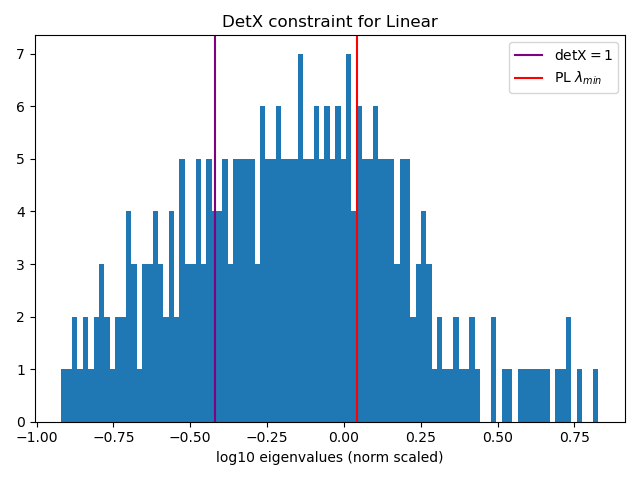
\includegraphics[width=5cm]{./img/detX_plots/LR=8/FC1/ww.layer3.detX.png}
        \label{fig:mlp3-randesd-8}
    }
    \subfigure[$LR=16\times$]{
      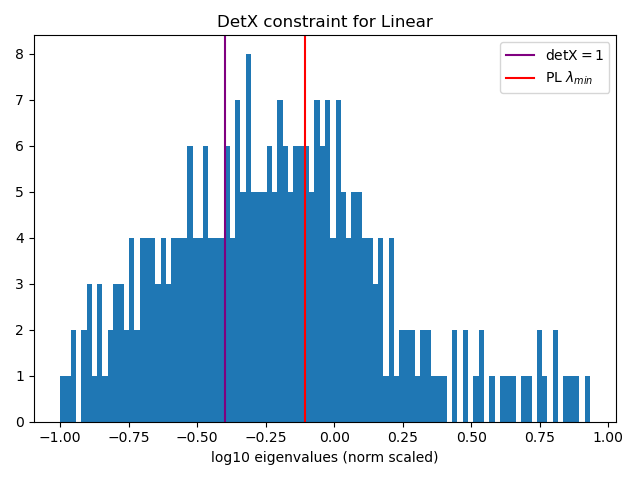
\includegraphics[width=5cm]{./img/detX_plots/LR=16/FC1/ww.layer3.detX.png}
        \label{fig:mlp3-randesd-16}
    }
    \subfigure[$LR=32\times$]{
      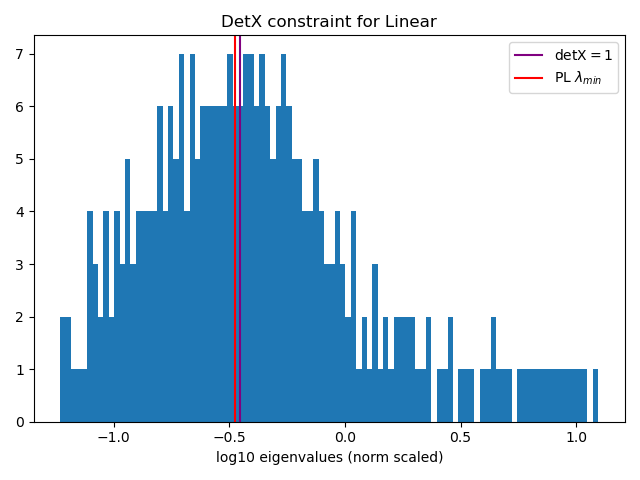
\includegraphics[width=5cm]{./img/detX_plots/LR=32/FC1/ww.layer3.detX.png}
        \label{fig:mlp3-randesd-32}
    }
    \caption{
        Log-Linear ESDs for three learning rates in the FC1 layer of MLP3. The red line shows $\LAMBDAPL$, and the 
        purple line shows $\LAMBDADETX$. Observe that the purple line is to the left of the red line, but as the LR 
        increases they move closer together. However, when LR is $32\times$, where both 
        train and test accuracy suffered (c), the red line is to the left of the purple line. This is often a signature 
        of an \OverRegularized layer, and indeed the FC1 layer in this model had $\alpha < 2$. (See Figure~\ref{fig:mlp3-alpha-fc1-by-lr} in 
        Section~\ref{sxn:empirical-test_acc}.)
    }
    \label{fig:mlp3-tracelognorm}
\end{figure}


We can compare  $\alpha$ and $\Delta \lambda_{min}$ more broadly by plotting $\Delta \lambda_{min}$ directly as a function of $\alpha$ in a single plot spanning all random seeds and learning rates or batch sizes.
This is shown in Figure~\ref{fig:mlp3-detx-gap}. 
Critical values of $\alpha=2$ and $\Delta \lambda_{min} = 0$ are shown as vertical and horizontal red lines, respectively. 
Values for various learning rates are plotted for layer FC1 
(Figure~\ref{fig:mlp3-detx-lr_search_fc1}) and FC2 (Figure~\ref{fig:mlp3-detx-lr_search_fc2}), as well as for various batch sizes in layer FC1 (Figure~\ref{fig:mlp3-detx-bs_search_fc1}) and FC2 (Figure~\ref{fig:mlp3-detx-bs_search_fc2}).

For layer FC1 (Figures~\ref{fig:mlp3-detx-lr_search_fc1} and~\ref{fig:mlp3-detx-bs_search_fc1}), in both cases we see near-linear march towards the critical tuple of $(\alpha, \Delta\lambda_{min}) = (2, 0)$.
In addition, passing this critical value coincides with diminished train and test accuracy, (recall 
Figure~\ref{fig:mlp3-accuracies}), suggesting that just as $\alpha=2$ is a threshold of over-regularization, $\LAMBDAPL < \LAMBDADETX$ may be as well. 
Since FC1 is the dominant layer, comprising roughly $8/9$ of the weights of the model, (Table~\ref{tab:mlp3},) we expect 
FC1 to most closely match the performance of the model as a whole.

For layer FC2, which comprises roughly the other $1/9$ of the models weights, there is a similar coevolution, but it is weaker. 
As learning rate or batch size exceeds their critical values, rather than going to $(2, 0)$ as in FC1, we instead see that the relationship simply breaks down, with the gap growing larger even as $\alpha$ decreases. 
Given that FC1 \emph{has} passed the critical $\alpha=2$ threshold, we conjecture that the breakdown of the relationship between $\alpha$ and $\Delta \lambda_{min}$ is due to FC1 becoming \ATypical.


\begin{figure}[t] %[h]
    \centering
    \subfigure[Layer FC1 for various learning rates]{
        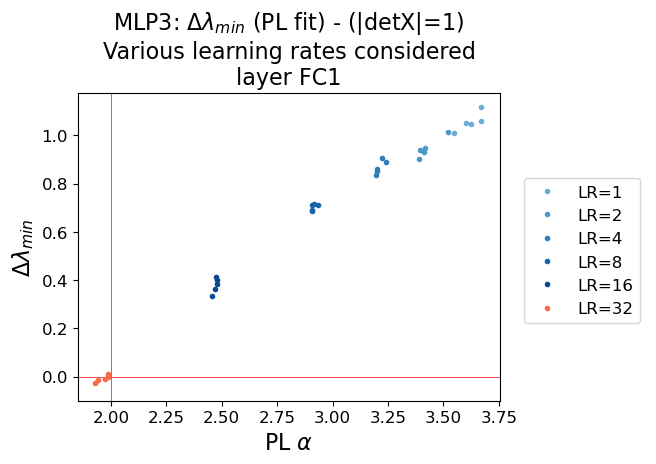
\includegraphics[width=7cm]{img/detX_plots/mlp3_detX_delta_LR_all_FC1.png}
        \label{fig:mlp3-detx-lr_search_fc1}
    }
    \subfigure[Layer FC2 for various learning rates]{
        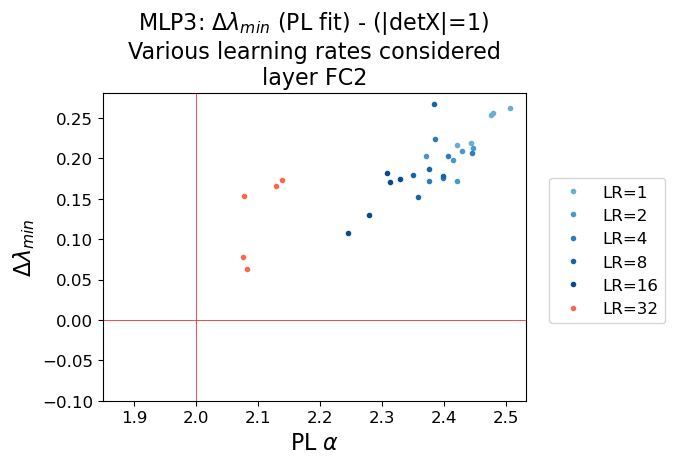
\includegraphics[width=7cm]{img/detX_plots/mlp3_detX_delta_LR_all_FC2.png}
        \label{fig:mlp3-detx-lr_search_fc2}
    }\\
    \subfigure[Layer FC1 for various batch sizes]{
        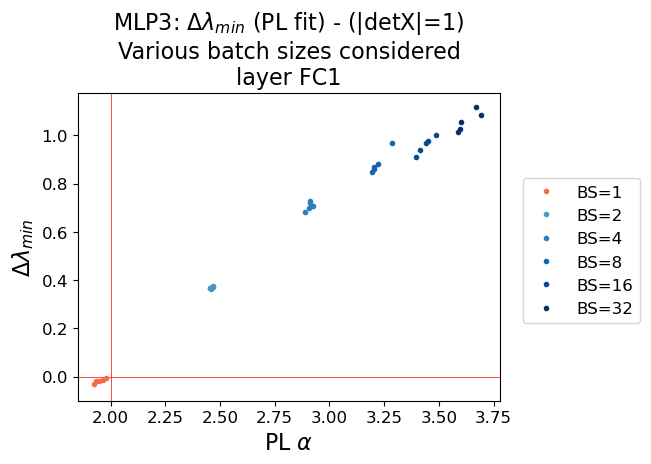
\includegraphics[width=7cm]{img/detX_plots/mlp3_detX_delta_BS_all_FC1.png}
        \label{fig:mlp3-detx-bs_search_fc1}
    }
    \subfigure[Layer FC2 for various batch sizes]{
        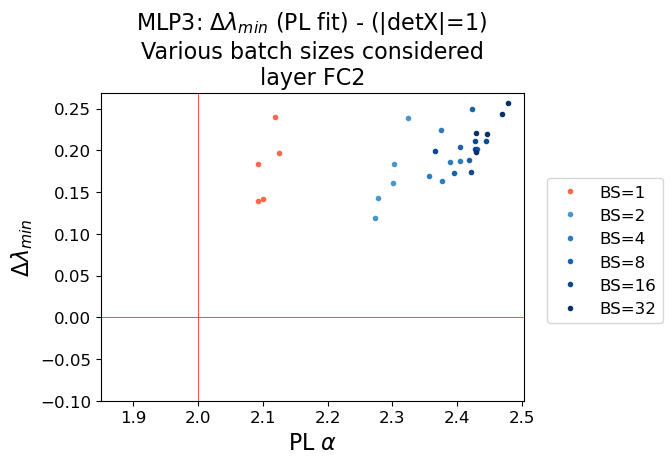
\includegraphics[width=7cm]{img/detX_plots/mlp3_detX_delta_BS_all_FC2.png}
        \label{fig:mlp3-detx-bs_search_fc2}
    }
    \caption{
            MLP3 Model: Comparison of the PL \ALPHA (x-axis), with the difference between $\LAMBDAPL$ and $\LAMBDADETX$ 
            (y-axis). The thin red lines indicate critical values of $\alpha=2$ and $\Delta \lambda_{min} = 0$. As 
            learning rate increases (a--b) or batch size decreases (c--d), we can see that in layer FC1, which dominates 
            the model, (See Table~\ref{tab:mlp3},) $\alpha$ goes to $2$, and $\Delta \lambda_{min}$ goes to $0$. Observe 
            that both critical values are crossed at the most extreme hyper-parameter selection, (red,) corresponding 
            with over-training. Layer FC2 shows a weaker tendency towards the critical values (b, d), and is disrupted 
            at the most extreme hyper-parameter values (red).
    }
 \label{fig:mlp3-detx-gap}
\end{figure}


\subsubsection{State-of-the-Art (SOTA) models}
\label{sxn:detx-sota}

Here, we consider SOTA models, 
in particular VGG pre-trained models~\cite{VGG14_TR}, the ResNet series~\cite{ResNet15_TR}, the ViT 
series~\cite{VIT20_TR}, and the DenseNet series~\cite{DenseNet17_TR}.
We show that as $\alpha$ approaches $2$, the Log-Trace Condition holds better and better, i.e., $\Delta\lambda_{min}$ 
approaches $0$.
%holds approximately for the PL portion of the tail
%even when $\alpha\gg2$ in some cases.

\begin{figure}[t] %[h]
    \centering
    \subfigure[VGG Series]{
      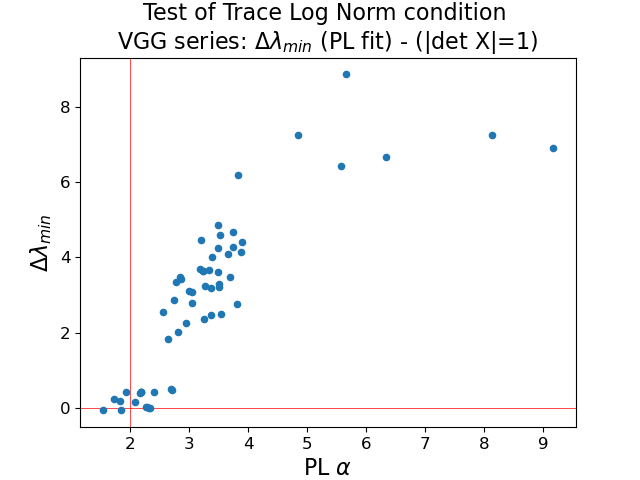
\includegraphics[width=7cm]{./img/VggTest.png}
      \label{fig:VGG_trend}
    }
    \subfigure[ResNet Series]{
      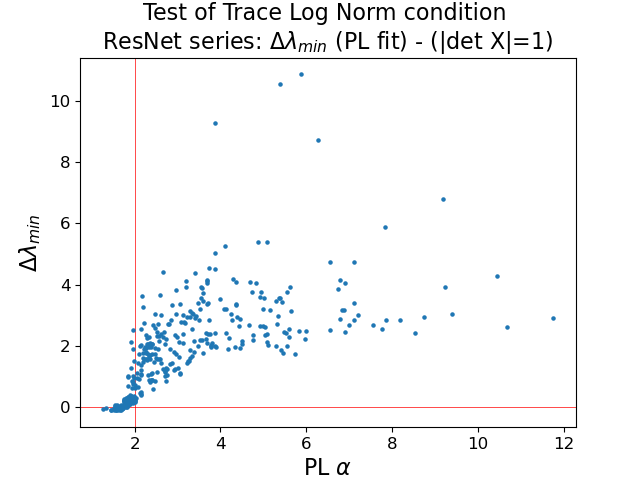
\includegraphics[width=7cm]{./img/ResNetTest.png}
      \label{fig:ResNet_trend}
    } \\
    \subfigure[ViT Series]{
      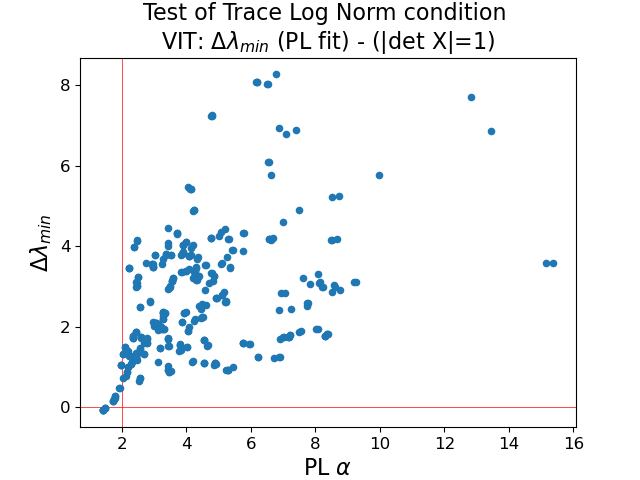
\includegraphics[width=7cm]{./img/VIT_ESD_trends.png}
      \label{fig:VIT_trend}
    }
    \subfigure[DenseNet Series]{
      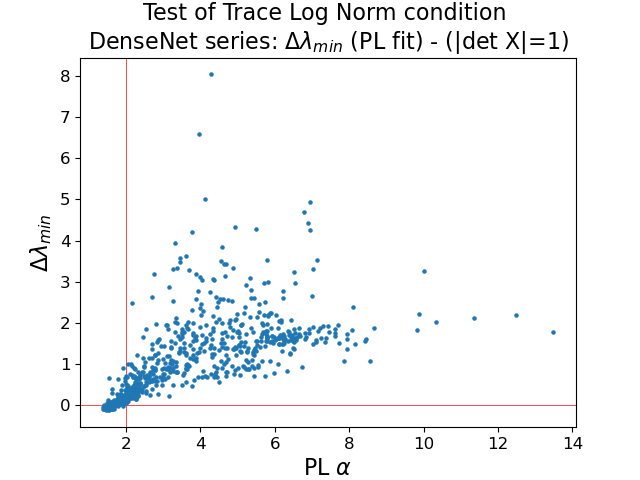
\includegraphics[width=7cm]{./img/DenseNetTest.png}
      \label{fig:DenseNet_trend}
    }
    \caption{Difference between the two $\lambda_{min}$ estimates, $\Delta\lambda_{min}$, (\EQN~\ref{eqn:D_lambda_min}), as a 
        function or $\alpha$, for linear and convolutional layers in series of VGG~\cite{VGG14_TR}, ResNet~ 
        \cite{ResNet15_TR}, ViT models~\cite{VIT20_TR} and DenseNet models~\cite{DenseNet17_TR}. Layer matrices for all 
        models in the series were pooled to create each plot. In (a), (VGG,) we see three clusters of points -- those 
        with $\Delta \lambda_{min}$ close to $0$ and $\alpha$ close to $2$, those with $\Delta \lambda_{min}$ above $2$ 
        and $\alpha > 2.5$, and those with $\Delta \lambda_{min}$ above $6$ and $\alpha > 3.5$. In (b), (ResNet,) we see 
        that in general, as $\alpha$ shrinks towards $2$, $\Delta \lambda_{min}$ tends towards $0$, overshooting 
        slightly. We also see that the difference $\Delta\lambda_{min}$ is almost always positive, with few exceptions, 
        and even the layers that do not overshoot form a kind of ``funnel shape pointing towards the critical point 
        $(2, 0)$. In (c), (ViT,) we also see the same general relationship between $\alpha$ and $\Delta \lambda_{min}$ 
        across layers of several ViT models. Observe that ViT models do not have convolutional layers, and in spite of 
        this, the overall pattern is similar. In (d), (DenseNet,) we see a similar overall trend as in (b), except that 
        $\Delta\lambda_{min}$ tends to decrease sooner, but there are also more layers with $\alpha < 2$ and 
        $\Delta\lambda_{min}$ above $0$.
    }
  \label{fig:CV_ESD_trends}
\end{figure}


Figure~\ref{fig:CV_ESD_trends} plots $\alpha$ versus the difference $\Delta\lambda_{min}$, (\EQN~\ref{eqn:D_lambda_min}).
Layer matrices from all models in each series are pooled to generate the plots.% 
\footnote{For convolutional layers, the \WW tool first computes eigenvalues for all channels-to-channels linear operators separately, and then pools them in order to compute $\alpha$, $\LAMBDAPL$ and $\LAMBDADETX$. For instance, in a $64\times 64\times 3\times 3$ weight tensor, there would be $9$ separate linear operators of $64\times 64$, giving $576$ eigenvalues, which would then be pooled to compute $\alpha$, $\LAMBDAPL$ and $\LAMBDADETX$.} 
Notice that in Figure~\ref{fig:VGG_trend} -- \ref{fig:DenseNet_trend}, $\Delta\lambda_{min}$ approaches zero as $\alpha\rightarrow 2$ from above. 
Individual points may have a large $\Delta\lambda_{min}$ for an $\alpha$ near to $2$, but the overall trend is apparent. 
The rapid decrease of $\Delta\lambda_{min}$ as $\alpha$ approaches $2$ from above implies that the PL tail rapidly 
takes on a unit \TRACELOG  (if it doesn't already have it.)

As we saw in comparison of Figures~\ref{fig:mlp3-msr-results-xmin} and~\ref{fig:mlp3-msr-results-detX}, 
(Section~\ref{sxn:trunc_err_epochs},) the \TRACELOG tail is generally larger, and always has highly generalizing 
components. Thus, it is plausible that as layers reach the limit of the amount of information that can be encoded in 
them, i.e. as $\alpha$ goes to $2$, the \POWERLAW~tail expands to fill the \TRACELOG tail. This effect can be seen 
clearly in Figure~\ref{fig:CV_ESD_trends} in the condensing of the ``funnel shape.

Recall from Figure~\ref{fig:mlp3-detx-gap} that layer FC1 dominated the model, (Table~\ref{tab:mlp3},) producing a clear 
progression of $\alpha$ and $\Delta\lambda_{min}$ towards $(2, 0)$, as a function of learning rate or batch size, whereas FC2 showed a slightly less clear relationship. 
In larger models having dozens or hundreds of layers, we would not expect any one layer to dominate as thoroughly.
Moreover, it is the architecture that varies between models in each series, not (necessarily) the hyperparameters, meaning that there would not be a straight line, as in Figures~\ref{fig:mlp3-detx-lr_search_fc1} and~\ref{fig:mlp3-detx-bs_search_fc1}. 
However, with all of the layers contributing to varying degrees, we nevertheless see a clear trend in all plots of Figure~\ref{fig:CV_ESD_trends}. 
These results show how the single-layer \SETOL theory extends from the MLP3 model, which is dominated by a single layer, to larger models where many layers interact in complex ways, but still reflect the same overall trend.


\begin{figure}[t] %[h]
    \centering
    \subfigure[Falcon 7B]{
      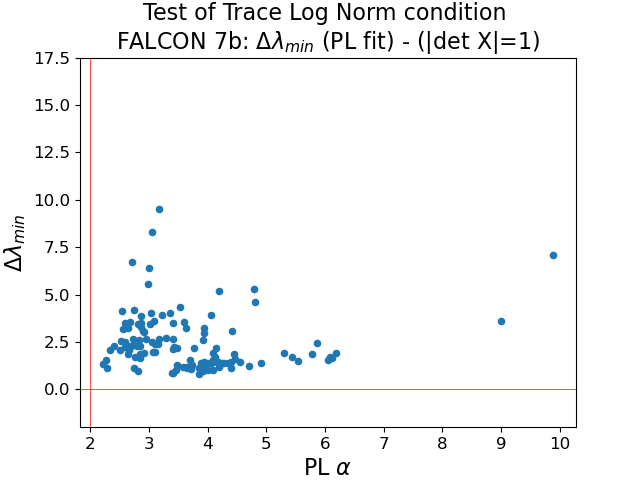
\includegraphics[width=7cm]{./img/FALCON7b_ESD_trends.png}
      \label{fig:falcon7B_trend}
    }
    \subfigure[Falcon 40B]{
      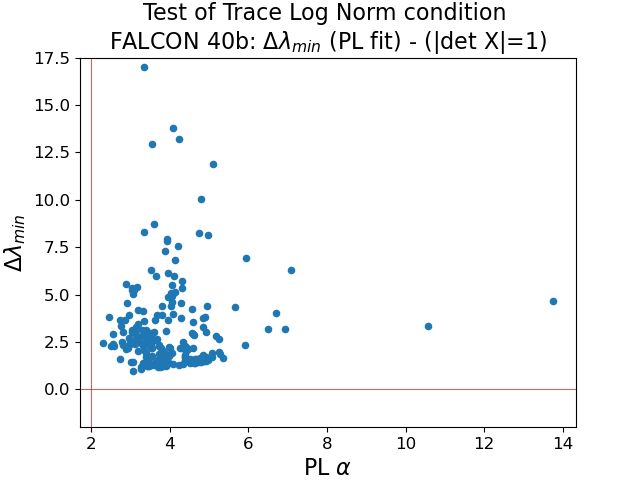
\includegraphics[width=7cm]{./img/FALCON40b_ESD_trends.png}
      \label{fig:falcon40B_trend}
    }
    \subfigure[Llama 13B]{
      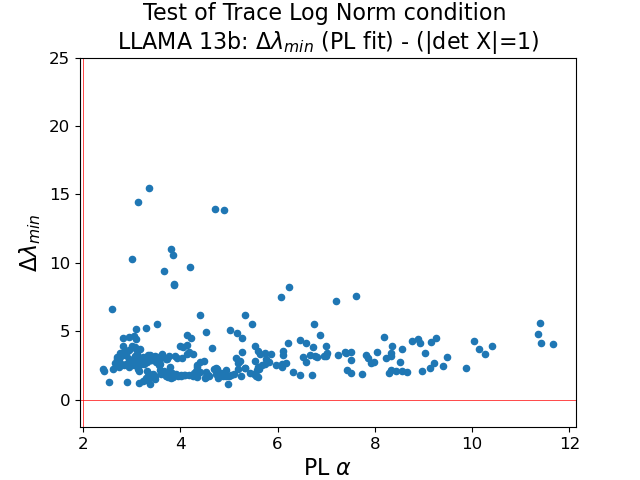
\includegraphics[width=7cm]{./img/LLAMA_13b_ESD_trends.png}
      \label{fig:llama13B_trend}
    }
    \subfigure[Llama 65B]{
      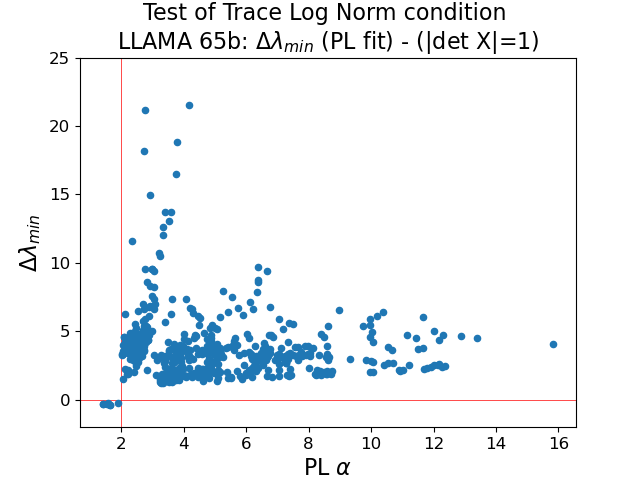
\includegraphics[width=7cm]{./img/LLAMA_65b_ESD_trends.png}
      \label{fig:llama65B_trend}
    }
    \caption{Difference between the two $\lambda_{min}$ estimates, $\Delta\lambda_{min} = \LAMBDAPL - \LAMBDADETX$, 
        as a function of $\alpha$, for all linear layers in the FALCON\cite{falcon40b}(a-b) and 
        LLAMA \cite{touvron2023_TR}(c-d) language models for varying numbers of parameters. As in Figure 
        \ref{fig:CV_ESD_trends}, we see that in recent Large Language Models, $\Delta\lambda_{min}$ remains positive, 
        except where $\alpha < 2$ (d). Otherwise, a ``funnel shape can still be seen leading towards the critical 
        point $(2, 0)$ as in Figures~\ref{fig:ResNet_trend} and~\ref{fig:VIT_trend} Observe that the x- and y-axes are 
        different between sub-figures due to the differences in scale of each model.
    }
  \label{fig:LLM_ESD_trends}
\end{figure}

The overall pattern of relationship between $\Delta\lambda_{min}$ and $\alpha$ can also be seen in 
Figure~\ref{fig:LLM_ESD_trends}, which shows plots for Large Language Models (LLMs) of the Falcon~\cite{falcon40b} and 
LLAMA~\cite{touvron2023_TR} model families, for different numbers of parameters. Observe that each 
subfigure~\ref{fig:falcon7B_trend}--\ref{fig:llama65B_trend} shows a single 
model, rather than a collection of models in a family, as in Figure~\ref{fig:CV_ESD_trends}.
The y-axis is the same between models in the same family. 
As in Figure~\ref{fig:CV_ESD_trends}, there is a general outline of a ``funnel shape pointing towards the critical 
point $(2, 0)$, with the exception that it is only reached in the case of LLAMA-65b, (Figure~\ref{fig:llama65B_trend}). 
This suggests that these LLMs are larger than they necessarily need to be, consistent with prior work~\cite{YHTx21_TR}, 
but also that they are well guarded against \OverRegularized layers beyond the critical point
($\alpha=2$ and $\Delta\lambda_{min}=0$).



\subsection{Model Quality: Computational \RTransforms}
\label{sxn:empirical_comp_r_transforms}

In this Section, we look at how the \HTSR layer quality HT PL metric $\alpha$
compares to computing the \LayerQualitySquared $\QT$ using
the Computational \RTransform method proposed in Section~\ref{sxn:comp_rmt}
for fully trained MLP3 model(s).
Figure~\ref{fig:MLP3_qualities}
presents results for FC1 and FC2 layers, comparing
both the batch size and the mean $\alpha$ metric to the
mean $\QT$, and the results are quite different.


\begin{figure}[t]
    \centering
    \subfigure[FC1 batch size vs $\QT$]{
        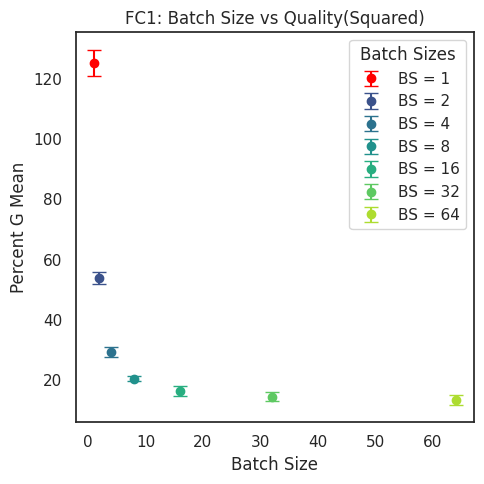
\includegraphics[width=6cm]{img/FC1_bs_vs_Q.png}
        \label{fig:FC1_bs_vs_Q}
    }
    \hspace{1cm} % Add space between subfigures
    \subfigure[FC1 Layer $\alpha$ vs $\QT$]{
        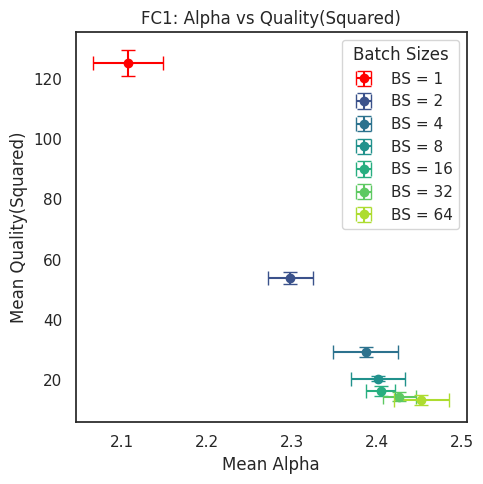
\includegraphics[width=6cm]{img/FC1_alpha_vs_Q.png}
        \label{fig:FC1_alpha_vs_Q}
    }
    \hspace{1cm} % Add space between subfigures
    \subfigure[FC2 batch size vs $\QT$]{
        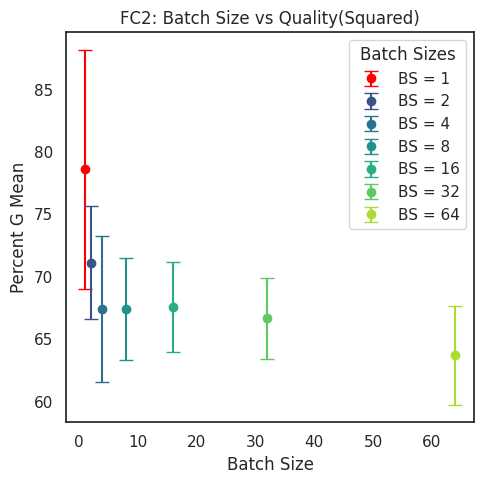
\includegraphics[width=6cm]{img/FC2_bs_vs_Q.png}
        \label{fig:FC2_bs_vs_Q}
    }
    \hspace{1cm} % Add space between subfigures
    \subfigure[FC2 Layer $\alpha$ vs $\QT$]{
        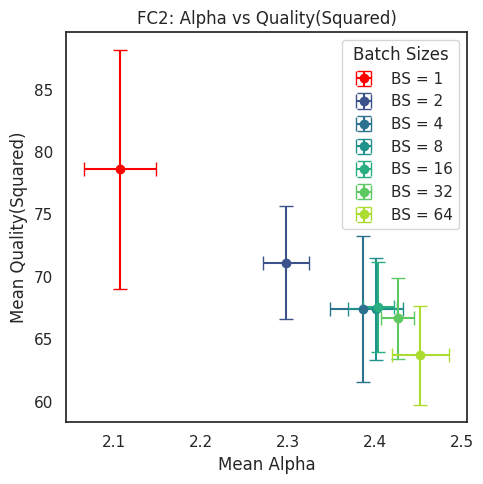
\includegraphics[width=6cm]{img/FC2_alpha_vs_Q.png}
        \label{fig:FC2_alpha_vs_Q}
    }
    \caption{
      Evaluation of the computational \RTransform \LayerQualitySquared metric $\QT$
      on the fully trained MLP3 model(s) for different batch sizes.
    }
    \label{fig:MLP3_qualities}
\end{figure}


For FC1, as shown in Figure~\ref{fig:FC1_bs_vs_Q}, the quality metric \(\QT\) increases as the batch size decreases, following the expected trend. Notably, for batch size = 1, the quality metric exceeds $100\%$,
which suggests that the layer may be overfit in this scenario, which is similar to results obtained earlier. Furthermore, in Figure~\ref{fig:FC1_alpha_vs_Q}, the quality metric \(\QT\) shows a strong correlation with the $\alpha$ metric, consistent with the theoretical predictions of the \HTSR framework.
Earlier results suggest that the FC1 layer captures most of the correlation in the data,
so it is interesting that this layer also has much smaller error bars, indicating more consistent computational
quality across different batch sizes.

In contrast, for FC2, while the general trends are similar (as shown in Figures~\ref{fig:FC2_bs_vs_Q} and~\ref{fig:FC2_alpha_vs_Q}), the error bars on the quality metric $\QT$ are much larger. This indicates significantly higher variability in computational quality compared to FC1. The large error bars for FC2 suggest that, while the $\QT$ metric is theoretically grounded, it is less effective than the existing \HTSR layer quality metric $\alpha$, which exhibits greater stability and reliability in capturing layer behavior. These differences highlight the distinct computational characteristics of the two layers, with FC1 demonstrating more predictable trends that align closely with theoretical expectations.




\subsection{Inducing a Correlation Trap}
\label{sxn:empirical-correlation_trap}

\begin{figure}[t]
    \centering
    \subfigure[MLP3 \LearningRate $16\times$]{
%        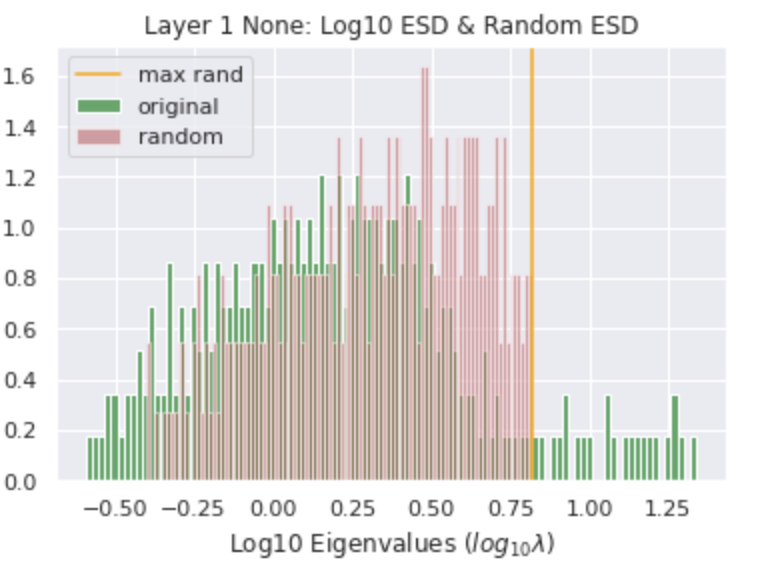
\includegraphics[width=6cm]{img/log-esd-bs2.png}
        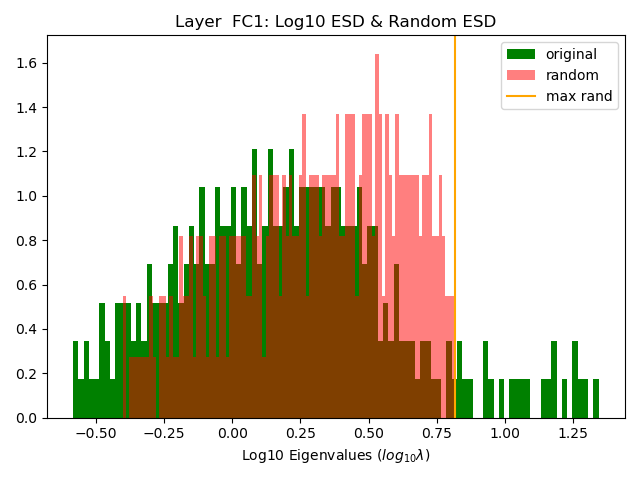
\includegraphics[width=6cm]{img/correlation_traps/LR_16_FC1_0/ww.layer3.randesd2.png}
        \label{fig:mlp3-accuracies3_lr16_trap}
    }
    \subfigure[MLP3 \LearningRate $32\times$]{
        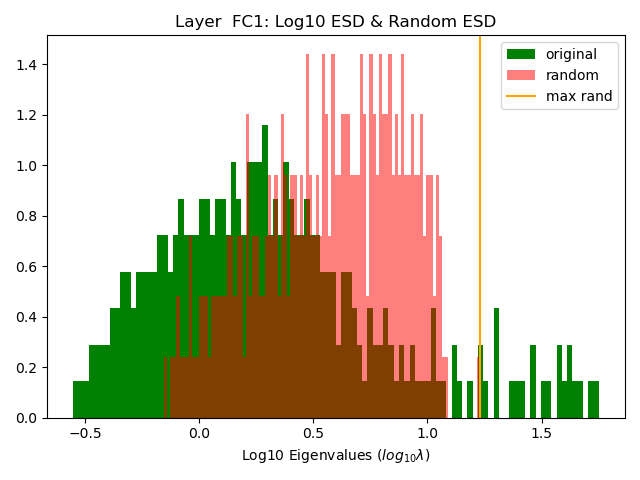
\includegraphics[width=6cm]{img/correlation_traps/LR_32_FC1_0/ww.layer3.randesd2.png}
        \label{fig:mlp3-accuracies3_lr32_trap}
    }
    \caption{ESD plots for learning rate $lr=16\times$ and $lr=32\times$ normal, shown on Log-Lin scale, as computed 
    using the \WW tool, for the FC1 weight matrix $\mathbf{W}$ (green) and an element-wise randomized $\mbox{rand}(\mathbf{W})$ (red).  
    This provides an example of inducing a \CorrelationTrap in the MLP3 model, simply by increasing the learning rate used during model training.  
        See Section~\ref{sxn:Traps}.
            }
    \label{fig:mlp3-accuracies3}
\end{figure}


Previous work on the \HTSR \Phenomenology \cite{MM20a_trends_NatComm,MM21a_simpsons_TR} has shown that one can look for 
quantitative deviations from the necessary pre-conditions of tradtitional \RMT (particularly that the weights are 
$0$-mean and finite variance) to detect when a model layer suffers from some other anomaly in the elements, which we 
call a ``\CorrelationTrap (see Section~\ref{sxn:Traps} and ~\cite{MM20a_trends_NatComm,MM21a_simpsons_TR}). A 
\CorrelationTrap may cause, or be caused by, the over-regularization leading \ALPHA to fall below $2$, (see 
Section~\ref{sxn:underfitting}). Here, we explore this in greater detail, in light of our \SETOL.

% Recall that a \CorrelationTrap arises when the randomized spectrum 
% is not an MP distribution. In this case, we know contrapositively that one or more of the MPs conditions on the 
% element-wise distribution ($0$-mean and finite variance) are not met. When the MP laws conditions are not met, we do 
% not have the usual guarantee that the element-wise distribution alone \emph{cannot} produce a large eigenvalue, meaning 
% that some of the large eigenvalues are likely not a result of correlations between pairs of data elements. 
%
Lets look at the ESDs of the FC1 layer of the MLP3 model, for learning rates $lr=16\times$ and $lr=32\times$ normal. 
We will be interested in the general shape of the ESD of $\tfrac{1}{N}\mathbf{W}^T\mathbf{W}$.
For the purposes of detecting a \CorrelationTrap, we will randomize $\mathbf{W}^T\mathbf{W}$ element-wise, and then observe its largest eigenvalue $\lambda^{max}_{rand}$. 
%%Randomizing element-wise is a way of drawing a sample random matrix whose elements are i.i.d.  from the same distribution as $\mathbf{W}^T\mathbf{W}$, so that any violations of the MP laws preconditions can be seen. 

Figure~\ref{fig:mlp3-accuracies3} shows the ESDs of the original matrix (green) and the element-wise 
randomized $\mbox{rand}(\tfrac{1}{N}\mathbf{W}^T\mathbf{W})$ (red). 
Observe in particular $\lambda^{max}_{rand}$ for each learning rate factor.
For $lr=16\times$, Figure~\ref{fig:mlp3-accuracies3_lr16_trap} shows 
that the ESD of $\tfrac{1}{N}\mathbf{W}^T\mathbf{W}$ is HT, whereas the ESD of the randomized matrix is essentially a distorted semi-circle---as expected from the well-known MP result; and 
that $\lambda^{max}_{rand}$ lies at the edge of the random \MPBulk ESD.
(A similar result is seen for smaller learning rates.)  
In contrast, for $lr=32\times$, Figure~\ref{fig:mlp3-accuracies3_lr32_trap} shows 
that while the original ESD is again HT, the ESD of the randomized has one large element, $\lambda^{max}_{rand}$, that pulls out from the MP bulk.
%
This is the signature of a \CorrelationTrap; and it co-occurrs with the exact learning rate setting that degraded the train and test accuracies, pushing \ALPHA below its optimal value of $\alpha\simeq 2$.
%
When this happens,  both the estimation of \ALPHA and the formation of a PL tail are potentially disrupted. 
%
%%Thus, by increasing the learning rate to $lr=32\times$ normal, we were able to systematically induce a \CorrelationTrap, 

\CorrelationTraps have been observed previously~\cite{MM20a_trends_NatComm,MM21a_simpsons_TR}, using the \HTSR \Phenomenology.
However, \SETOL provides an explanation for why this would be expected to occur --- non-standard element-wise distributions will tend to interfere with the properties of the spectrum which \SETOL analyzes. 
Our derivation in Section~\ref{sxn:empirical} suggests that in order to apply the \SETOL effectively one must avoid (or remove) such traps. 
This too has been observed previously~\cite{MM20a_trends_NatComm,MM21a_simpsons_TR}. 


%\chris{There was some old discussion on alphahat that I have commented here.}
%Notice that, in Figure~\ref{fig:mlp3-accuracies2_mlp3-alphahat},
%and in contrast to \ALPHA, however, the \ALPHAHAT value for $bs=1$ is larger, not smaller,
%and almost follows the trend the other values show.   This happens because
%the \ALPHAHAT metric corrects for the anomalous \Scale in the $bs=1$ case.
%Since $\ALPHAHATEQN=\alpha\log_{10}\lambda_{max}$, the metric multiplies the spuriously
%small $\alpha$ by the spuriously large $\log_{10}\lambda_{max}$, and there
%is a fortuitous cancellation of errors.  This is, in part, why the (layer averaged)
%\ALPHAHAT can describe trends in the quality of models when using just \ALPHA fails.




\subsection{Overloading and the Hysteresis Effect}
\label{sxn:hysteresis_effect}

%Here, we do such-and-such. 
%XXX.  HOW PRECISELY TO FRAME.

\michaeladdressed{This par should go somewhere.  Where?}
\charles{@michael: again, no changes to section 6}
Obtaining a value of $\alpha$ outside the $\alpha \gtrsim 2$ range is indicative of ``overloading~\cite{SST92} that layer. 
This can be accomplished, e.g., by training only one layer in the MLP3 model.
As the two layers have very different sizes, we see markedly different behaviors, that are nevertheless consistent with theory.

The \SETOL theory is based on the idea that NNs undergoing training behave like Statistical Mechanic systems relaxing to an equilibrium. 
So far, we have tested the theory under conditions that are approaching \Ideal. 
However, for the theory to be useful in practice, we must also examine how it performs in non-\Ideal situations. 
Of particular interest, we would like to examine the theory under conditions where the training dynamics slows down, i.e., when it is in a ``glassy''
or meta-stable state. 
One way we can do this is to train only one layer, and freeze the rest. 
Doing so overloads the single trainable weight matrix, as a function of the ratio of examples to trainable
parameters~\cite{SST92,Gardner_1988,MM17_TR}, and we expect this to cause $\alpha_{FC1}$ or $\alpha_{FC2}$ to drop well below $2$. As in \ref{sxn:empirical-effective_corr_space}, we will be examining this effect over the entire course of training.

\michaeladdressed{@chris: reorganize the figures in this section, like we discussed.  Also, organie the text properly into each subsubsection.}
\chris{Ive split the figures and re-organized. Lets discuss.}

\subsubsection{Baseline: Loading onto both FC1 and FC2}
\label{sxn:hysteresis_baseline}
\begin{figure}[t] %[h]
    \centering
%    \subfigure[FC1 \ALPHA vs train and test error]{
        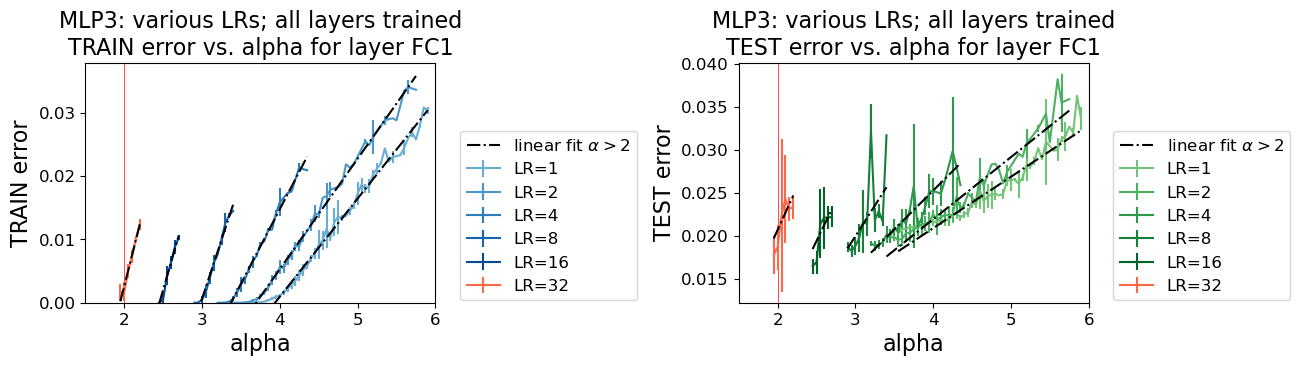
\includegraphics[width=15cm]{img/alpha_by_scales/mlp3_error_by_LR_all_FC1_binned.png} \\
%        \label{fig:mlp3-FC1-alpha-all-trained}
%    }\\
    \begin{tabular}{ccc}
      (a)\hspace{5cm} & (b) 
    \end{tabular}
%    \subfigure[FC2 \ALPHA vs train and test error]{
        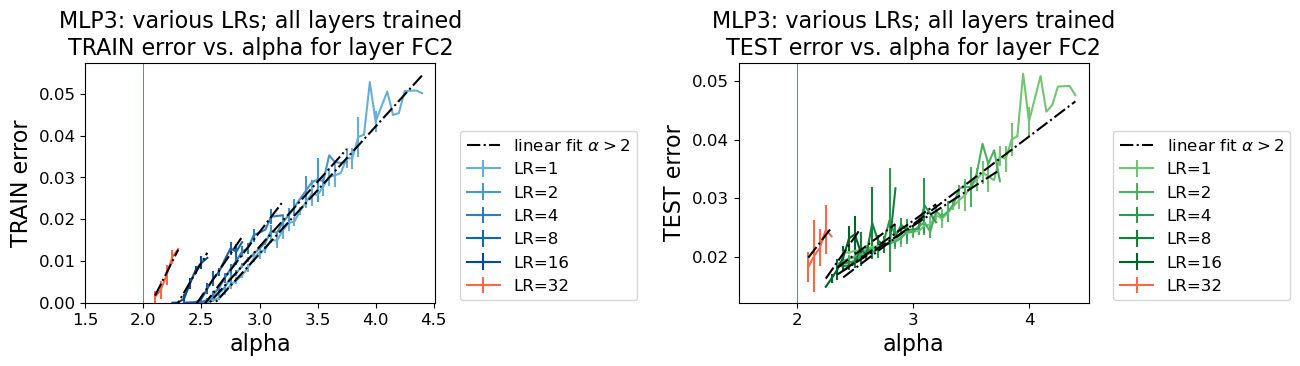
\includegraphics[width=15cm]{img/alpha_by_scales/mlp3_error_by_LR_all_FC2_binned.png}
%        \label{fig:mlp3-hyst-all-FC2-LR32}
%    }
    \begin{tabular}{ccc}
      (c)\hspace{5cm} & (d) \\
    \end{tabular}
    \caption{
        Train (a, c) and test (b, d) accuracy as a function of $\alpha_{FC1}$ (a, b) and $\alpha_{FC2}$ (c, d) when {\bf all 
        layers are trained}. Red vertical lines show the critical value of $\alpha = 2$, and dashed black lines show 
        linear fits of error, using only points where $\alpha > 2$ and train error $> 0.001$. 
        For FC1 (a, b), we can see that each learning rate 
        produces a different trajectory of train error (a) and test error (b) as a function of $\alpha_{FC1}$, 
        showing that even though FC1 dominates overall, (Table~\ref{tab:mlp3},) FC2 still plays a modulating role. 
        (Cf. Figure~\ref{fig:mlp3-FC1-alpha-overloaded} where there is only one trajectory.)
        In (c, d) we can see that $\alpha_{FC2}$ never goes below $2$. As in (a, b), each learning rate 
        produces a different trajectory, though there is greater overlap for lower learning rates. See discussion in 
        Section~\ref{sxn:hysteresis_baseline}.
    }
    \label{fig:mlp3-baseline-load}
\end{figure}


%\michaeladdressed{Backpoint explicitly to what figs/section is being referred to here.} Done

To start, Figure~\ref{fig:mlp3-baseline-load} shows $\alpha_{FC1}$ and $\alpha_{FC2}$, binned in units of $0.05$, versus 
train and test error over all epochs of training
\footnote{Excluding the first four epochs when the matrix is still essentially random.} 
for each of the different learning rates considered. 
(Cf. Figures~\ref{fig:mlp3-alphas-lr} and~\ref{fig:mlp3-alphas-bs}, Section~\ref{sxn:empirical-effective_corr_space},
which show only the final epoch.)
Binning was done so as to facilitate averaging over the $5$ starting random seeds; 
linear fits are shown separately for each learning rate; and
error bars represent one standard deviation within each bin. 
The critical value of $\alpha=2$ is shown as a vertical red line in all plots. 
For each learning rate, train error and $\alpha$ decrease together during training, which can be seen for both 
$\alpha_{FC1}$ (a) and $\alpha_{FC2}$ (c), reading each line from the top right to bottom left. Test errors, (b, d) show 
a similar trend, but with wider error bars. 
Observe that the range of the y-axis is narrower for test error to make detail more visible.
\chris{CH TODO: Double check these plots. The y-axis should be the same vertically.}

We see in Figure~\ref{fig:mlp3-baseline-load} (a,b) 
\michaeladdressed{soft-code, dont hard-code subfigure references}
\chris{Splitting these figures is manual, so the soft-coding is a stand-in until they are finalized and frozen.}
that the $32\times$ learning rate causes $\alpha_{FC1}$ to decrease faster than any other, putting it on course to 
fall below $2$ before train error reaches $\simeq 0$. 
(See Figure~\ref{fig:mlp3-accuracies}, at the beginning of this Section.) 
We also see that the slower learning rates cause train error to reach $\simeq 0$ well before $\alpha_{FC1}$ can reach $2$, and explains as to why their test error was higher.

%the FC1 layer, which has been shown to dominate 
%learning -- test error behaves more concordantly with FC1 $\alpha_{FC1}$. With FC1 frozen to its initial random state, the 
%much smaller FC2 will have to do all of the learning. 


\subsubsection{Overloading FC1}
\label{sxn:hysteresis_effect_FC1}


\begin{figure}[t] %[h]
    \centering
%    \subfigure[FC1 \ALPHA vs train and test error]{
        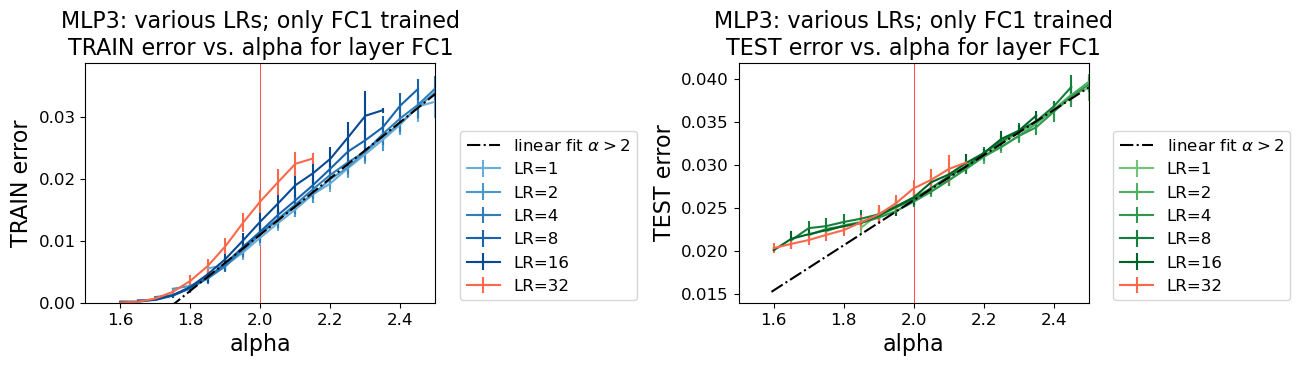
\includegraphics[width=15cm]{img/alpha_by_scales/mlp3_error_by_LR_FC1_FC1_binned.png}
%        \label{fig:mlp3-FC1-alpha-FC1-trained}
%    }
    \begin{tabular}{ccc}
      (a)\hspace{5cm} & (b) \\
    \end{tabular}
    \caption{
            Train and test accuracy as a function of $\alpha_{FC1}$ when only FC1 is trained (a, b). 
            Red vertical lines show the critical value of $\alpha_{FC1} = 2$, and dashed black lines show 
            linear fits of error, using only points where $\alpha_{FC1} > 2$. 
            In contrast with Figure~\ref{fig:mlp3-baseline-load}, when only 
            FC1 is trained, we can see that no matter the learning rate, there is ony one trajectory, for both train 
            error (a) and test error (b). Hence, for visibility, only one linear fit, using all learning rates pooled, 
            is shown. Crucially, we can see in (b) that as $\alpha_{FC1}$ passes below $2$, the \emph{test error} 
            trajectory changes, for all learning rates, even as the \emph{train error} trajectory does not, until it 
            reaches $\sim 0$. This suggests that even though test accuracy can still decrease when $\alpha_{FC1} < 2$, it 
            does so at a decreased rate relative to $\alpha_{FC1}$. See discussion in 
            Section~\ref{sxn:hysteresis_effect_FC1}.
    }
    \label{fig:mlp3-FC1-alpha-overloaded}
\end{figure}


In contrast, when only FC1 is trained, Figure~\ref{fig:mlp3-FC1-alpha-overloaded} shows that, as expected, 
$\alpha_{FC1}$ decreases well below $2$. Training error (a) generally trends downward as $\alpha_{FC1}$ decreases, 
but no matter the learning rate, the relation is the same, or nearly so, because only one layer is being trained. 
Consequently, all learning rates were pooled to produce one linear fit for enhanced visibility.

In Figure~\ref{fig:mlp3-FC1-alpha-overloaded} we can see 
demonstration of a crucial claim of \SETOL theory: that for $\alpha_{FC1} > 2$, (vertical red line,) the test 
error declines linearly; (b) shows that test error is almost perfectly linear with decline in $\alpha_{FC1}$. However, when $\alpha_{FC1} < 2$, the curve bends 
upward. 
Furthermore, the precision with which the trajectory changes as $\alpha_{FC1}$ passes the threshold provides ample 
validation that the estimator of~\cite{CSN09_powerlaw} is indeed accurate. We 
observe that test error may continue to decrease after $\alpha_{FC1} < 2$, however the rate of decrease is significantly less. 
We can also see that in some sense, the model is ``doomed'' to always have train error reach $\simeq 0$ when 
$\alpha_{FC1} \simeq 1.7$, i.e., after $\alpha = 2$, because of the number of trainable parameters, and perhaps because 
of the lack of a modulating influence of FC2 seen in Figure~\ref{fig:mlp3-baseline-load}.

\chris{This might be a good place to cite Temperature Balancing, Layer-wise Weight Analysis, and Neural Network Training because this corroborates the idea that learning rates work differently on different layers.}\michael{Yes.}
\charles{@michael: do it then!}


%In the FC1 layer we see that as $\alpha$ decreases below $2$, the rate of 
%decrease of test error begins to slow down at exactly that point. In FC2, which has much less capacity for storing 
%patterns, we see a different behavior resembling a Hysteresis curve\cite{???}. We also observe a point beyond which the 
%different random seeds show markedly different behavior which we conjecture is a result of \Replica Symmetry 
%Breaking\cite{SST92}.


\subsubsection{Overloading FC2}
\label{sxn:hysteresis_effect_FC2}

\begin{figure}[t] %[h]
    \centering
%    \subfigure[FC2 \ALPHA \LearningRate $16\times$]{
        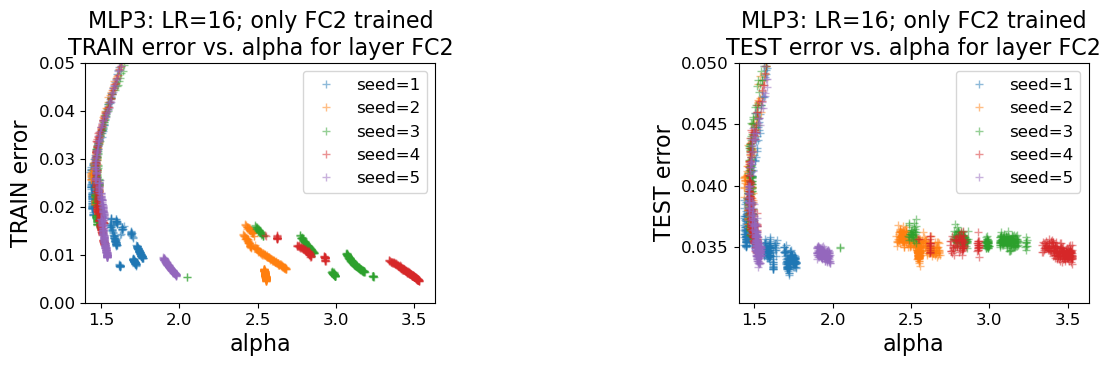
\includegraphics[width=15cm]{img/alpha_by_epochs/mlp3_error_by_LR=16_FC2_FC2.png}
%        \label{fig:mlp3-hyst-FC2-FC2-LR16}
%    }\\
    \begin{tabular}{ccc}
      (a)\hspace{5cm} & (b) \\
    \end{tabular}
%    \subfigure[FC2 \ALPHA \LearningRate $32\times$]{
        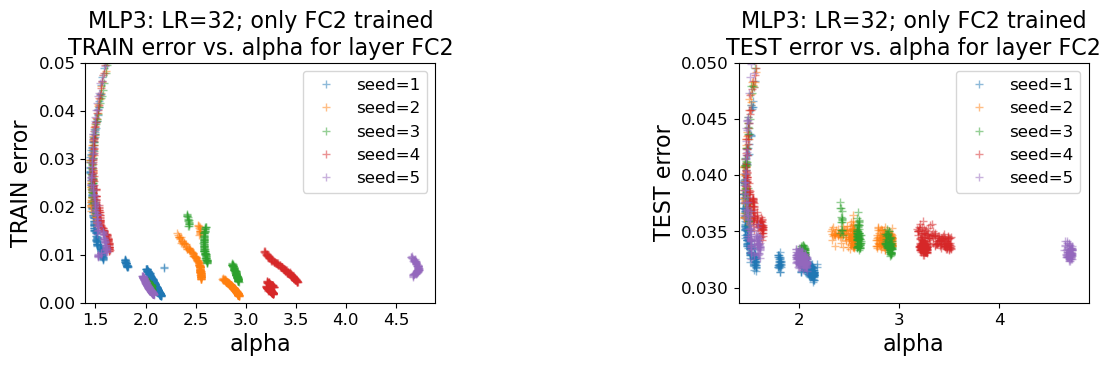
\includegraphics[width=15cm]{img/alpha_by_epochs/mlp3_error_by_LR=32_FC2_FC2.png}
%        \label{fig:mlp3-hyst-FC2-FC2-LR32}
%    }
    \begin{tabular}{ccc}
      (c)\hspace{5cm} & (d) \\
    \end{tabular}
        \caption{Train error (a, c) and test error (b, d) as a function of $\alpha_{FC2}$ when all other layers are 
        frozen, for the two largest learning rates, $lr=16\times$, (a, b) and $lr=32\times$(c, d). Cf. 
        Figure~\ref{fig:mlp3-baseline-load}, wherein all layers were trained. Due to the markedly different 
        behavior of each random seed, they cannot be plotted as means and error bars, and are instead shown separately. 
        The path taken by all seeds up to $\alpha_{FC2} = 1.5$ has a slight curvature characteristic of a 
        hysteresis-like behavior. Observe also that the fragmenting into separate paths, due to the breakdown of the 
        PL tail, coincides roughly with each seeds path reaching its minimum test error. The y-axis is scaled 
        differently for train and test error to make variation more visible. See discussion in 
        Section~\ref{sxn:hysteresis_effect_FC2}.
    }
    \label{fig:mlp3-FC2-alpha-hysteresis}
\end{figure}

\michaeladdressed{This par maybe should go into the baseline subsection above.}
\chris{See my changes.}
The MNIST dataset has $60,000$ training examples, which means that an FC1-only model is over-parameterized, but FC2 is 
substantially \emph{under}-parameterized~\cite{DLM19_Exact_TR}. (Table~\ref{tab:mlp3}) This drastically changes the 
meaning of an experiment where only FC2 is trained. Figure~\ref{fig:mlp3-baseline-load} (Section 
\ref{sxn:hysteresis_baseline}) shows $\alpha_{FC2}$ vs. train error (c) and test error (d) when \emph{all} layers are 
trained. There we see a different relationship between $\alpha_{FC2}$ and train and test error for each learning rate. 
None of the training runs reached an $\alpha_{FC2}$ of $2$, as the load was split between both layers FC1 and FC2.

Figure~\ref{fig:mlp3-FC2-alpha-hysteresis}, however, shows a starkly different relationship. 
\michaeladdressed{We need to show more, especially earlier in training, so its clear that the curves are similar and then split.}
\charles{@michael: Chris has moved on and we need to work with what we have}
When only FC2 is trained, 
each random seed produces a different trajectory, meaning that they cannot be interpretably plotted as a single curve, even with error 
bars. Train (a, c) and test (b, d) error rates are shown as a function of $\alpha_{FC2}$ for the two highest learning 
rate factors, $16\times$ (a, b) and $32\times$ (c, d). Lower learning rate factors, (not shown,) showed the same trend, except 
that they did not progress as far as those shown in Figure~\ref{fig:mlp3-FC2-alpha-hysteresis}.
\michaeladdressed{Not clear.}
\charles{@michael: this should have been addressed a year ago}

First we see, for all seeds, $\alpha_{FC2}$ decreases all the way down to $1.5$, after which it begins to rebound to the 
right. As it 
does, train error continues to decrease. We can also see that test error continues to decrease as well, down to its minimum 
value of slightly more than $0.03$, as $\alpha_{FC2}$ continues to increase for a short time. However, at the exact 
point where test error reaches a minimum, the PL tail itself begins to fracture, leading to different estimates 
of $\alpha_{FC2}$ for each seed. As each of the five starting random seeds are shown separately, we can see that each of 
them terminates at a different point, some of which are closer to $2$ than others.

Such a reversion to a more \Typical value of $\alpha_{FC2}$, prior to the fracturing of the PL tail, is 
reminiscent of a spin glass system relaxing towards its minimum energy configuration, in a way that retains some memory 
of the path taken on the way to its current state. 
\michaeladdressed{We show fracturing, then claim it is \ATypical, but we dont show hysterisis, which is the title of the subsection.  We should show that explicitly to be more clear.}
\chris{The claim of hysteresis is based on the bending seen in the curve (left, top to bottom,) just before fracturing 
        happens. We can also see that though the curves fracture, they all continue bending strongly to the right.
        The theory predicts that alpha will decrease, but it doesnt predict that it will rebound as we see there. The 
        only mechanism we know of that would predict such bending, seen most clearly in (a, c), is hysteresis.
}
We conjecture that if the model were trained for sufficiently many 
epochs, (perhaps many thousands,) then the tail would re-form, and $\alpha_{FC2}$ would reform, and revert all the way back to its 
stable value of $2$.


